\documentclass[a4paper,11pt]{article}
\usepackage[T1]{fontenc}		% Seleção de códigos de fonte
\usepackage[utf8]{inputenc}		% Codificação do documento (conversão
\usepackage{indentfirst}		% Indenta o primeiro parágrafo de cada seção.
\usepackage{graphicx}			% Inclusão de gráficos
\usepackage{subcaption}				% enables the use of subfigures in floats
\usepackage[
%	a4paper,
left=2cm,
right=1.5cm,
bottom=1.5cm,
top = 2.5cm, 
foot=0.7cm]{geometry}
\usepackage{url}
\usepackage{setspace}
\usepackage{amsmath}
\usepackage{amsfonts}
\usepackage{fancyhdr}
\usepackage{multirow}
\usepackage{tabularx}
\usepackage{natbib}
\usepackage{import}
\usepackage[nottoc]{tocbibind} % insere as referências no sumário
\usepackage[brazil]{babel}
\usepackage{hyperref}
\usepackage{float}

\pagestyle{fancy}
\fancyhf{}
\lhead{EEL5193 - Máquinas e Acionamentos Elétricos para Automação}
\rhead{Trabalho 1}
\rfoot{\thepage}

\begin{document}
	\thispagestyle{empty}
\begin{center}
	
\includegraphics[height=2cm]{imagens/logoUFSCsimples.png} \\
	{\Large Universidade Federal de Santa Catarina -- UFSC} \\
	{\Large Centro Tecnológico -- CTC} \\
	{\Large Departamento de Automação e Sistemas -- DAS} \\
	\vspace{1cm}
	{\large Disciplina DAS 5310 - Avaliação de Desempenho de Sistemas de Automação Discretas} \\
	\vfill
	\large{\textbf{Relatório do Trabalho ARENA} \\
	} 
	\vspace{1cm}
	% Integrantes: \\
    Bruno Machado Pacheco (16100865) \\
    \vfill
	Florianópolis, \today.
\end{center}

\clearpage

\tableofcontents

\clearpage

%%%%%%%%%%%%%%%%%%%%%%%%%%%%%%%%%%%%%%%%%%%%%%%%%%%%%%%%%


Uma máquina de corrente contínua pode funcionar tanto como um gerador, convertendo energia mecânica em energia elétrica, quanto como um motor, convertendo energia elétrica em mecânica. Apesar de a energia elétrica ser comumente distribuída (no nível do consumidor) em corrente alternada, os motores de corrente contínua possuem grande participação na indústrias, uma vez que permitem facilmente a variação de velocidade, por exemplo, de uma esteira ou um comboio. 

Por outro lado, componentes eletrônicos de tensão alternada, cada vez mais acessíveis, são capazes de controlar a velocidade de motores assíncronos da mesma forma, logo, pelo seu melhor custo benefício, eles vêm substituindo os motores de corrente contínua na maior parte das aplicações. De toda forma, o estudo dos motores de corrente contínua é fundamental pois introduz os conceitos básicos do funcionamento de máquinas elétricas. A figura \ref{fig:MCC} mostra esquematicamente uma máquina de corrente contínua elementar.

\begin{figure}[ht!]
\center
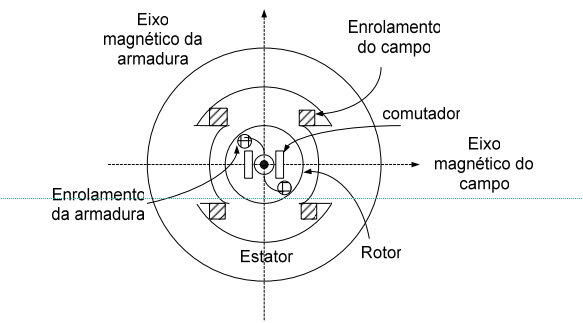
\includegraphics[scale=0.66]{imagens/maquina_cc.png}
\caption{\label{fig:MCC}Máquina de corrente contínua elementar.}
\caption*{Fonte: Máquinas de corrente contínua \protect\footnotemark}
\end{figure}

\footnotetext{Disponível em: <http://www.gsep.ene.unb.br/osem/ivan/Conversao> Acesso em out. 2018.}


\newpage

\section{Retificadores}


Uma máquina de corrente contínua pode funcionar tanto como um gerador, convertendo energia mecânica em energia elétrica, quanto como um motor, convertendo energia elétrica em mecânica. Apesar de a energia elétrica ser comumente distribuída (no nível do consumidor) em corrente alternada, os motores de corrente contínua possuem grande participação na indústrias, uma vez que permitem facilmente a variação de velocidade, por exemplo, de uma esteira ou um comboio. 

Por outro lado, componentes eletrônicos de tensão alternada, cada vez mais acessíveis, são capazes de controlar a velocidade de motores assíncronos da mesma forma, logo, pelo seu melhor custo benefício, eles vêm substituindo os motores de corrente contínua na maior parte das aplicações. De toda forma, o estudo dos motores de corrente contínua é fundamental pois introduz os conceitos básicos do funcionamento de máquinas elétricas. A figura \ref{fig:MCC} mostra esquematicamente uma máquina de corrente contínua elementar.

\begin{figure}[ht!]
\center
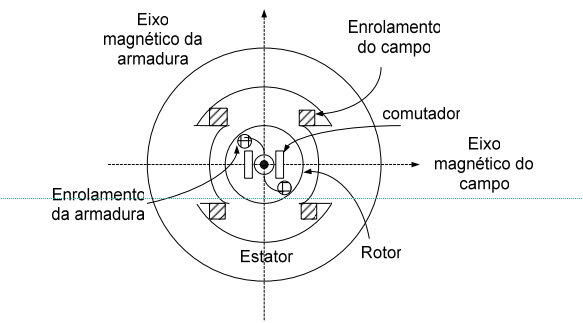
\includegraphics[scale=0.66]{imagens/maquina_cc.png}
\caption{\label{fig:MCC}Máquina de corrente contínua elementar.}
\caption*{Fonte: Máquinas de corrente contínua \protect\footnotemark}
\end{figure}

\footnotetext{Disponível em: <http://www.gsep.ene.unb.br/osem/ivan/Conversao> Acesso em out. 2018.}



\subsection{Retificadores a Diodo}

Retificadores a diodo se utilizam da capacidade desse semicondutor de permitir a passagem corrente de forma unidirecional, desde que sejam respeitados os seus limites de operação.

\subsubsection{Retificadores monofásicos de meia onda}


No caso monofásico, o retificador de meia onda associa somente um diodo na saída de tensão da fonte. Dessa forma, somente em um dos semiciclos (geralmente o positivo) da tensão alternada de alimentação $v\left( \omega t \right) $ há passagem de corrente para a carga.

No caso de uma carga resistiva pura, a estrutura do retificador monofásico de meia onda pode ser visto na figura \ref{fig:RMMOCR}.

\begin{figure}[htb]
\center
\includegraphics[scale=0.55]{imagens/RetifMeiaOndaCargaResistiva.png}
\caption{Retificador monofásico de meia onda com carga resistiva.}
\label{fig:RMMOCR}
\end{figure}

Como mencionado acima, o diodo bloqueia o semiciclo negativo da tensão alternada, portanto a tensão aparente para a carga $R$ consiste somente dos semiciclos positivos.

Sendo a tensão de alimentação \[
v(\omega t)=\sqrt{2}V_o\sin(\omega t) 
\] podemos calcular a tensão média na carga
\begin{align*}
    V_{L,med} &= \frac{1}{2\pi}\int_\alpha^{\pi}\sqrt{2}V_o\sin(\omega t)d(\omega t) \\
	     &= \frac{\sqrt{2}V_o}{2\pi}[-\cos(\omega t)]_\alpha^{\pi} \\
	     &\approx 0,45 V_o
.\end{align*}

A corrente média na carga, então, é
\begin{align*}
    I_{L,med} &= \frac{1}{2\pi}\int_\alpha^{\pi}\frac{\sqrt{2}V_o}{R}\sin(\omega t)d(\omega t) \\
    &= \frac{V_{L,med}}{R} \\
    &\approx \frac{0,45 }{R}V_o
.\end{align*}


A corrente de pico no diodo $I_{D,p}$ é tal qual a corrente de pico na carga, ou seja, \[
I_{D,p} = \frac{\sqrt{2}V_o}{R}
,\] enquanto a tensão de pico inversa do diodo é \[
    V_{D,p} = \sqrt{2}V_o
.\] 

Para o dimensionamento correto do diodo é necessário saber o valor eficaz da corrente que passa por ele, ou seja,
\begin{align*}
    I_{L, ef} &= \sqrt{\frac{1}{2\pi} \int_{\alpha}^{\pi}\left(  \frac{\sqrt{2}V_o}{R}\right) ^{2}\sin^{2}(\omega t)d(\omega t)} \\
&=\sqrt{\frac{V_o^{2}}{\pi R^{2}}\int_{\alpha}^{\pi}\sin^2(\omega t)d(\omega t)} \\
&= \frac{V_o}{\sqrt{2}R} \approx 0.707\frac{V_o}{R}
.\end{align*}

No caso de uma carga RL com componente indutivo, a estrutura do retificador monofásico de meia onda pode ser vista na figura \ref{fig:RMMOACRL}.

\begin{figure}[h]
\center
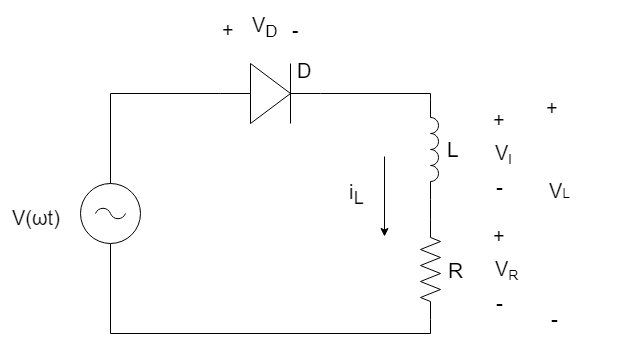
\includegraphics[scale=0.55]{imagens/cargaRl.png}
\caption{Retificador monofásico de meia onda com carga com componente indutivo}\label{fig:RMMOACRL}
\end{figure}

Agora, devido à indutância, há uma defasagem entre a corrente e a tensão, então o diodo não mais impede a passagem de corrente quando $\omega t = \pi$, mas em um ângulo $\beta$ maior do que $\pi$, como observado na figura \ref{fig:FO}. Ou seja, enquanto a corrente não se anula, o diodo continua conduzindo e, portanto, a tensão na carga torna-se negativa para ângulos superiores a $\pi$.

\begin{figure}[h]
\center
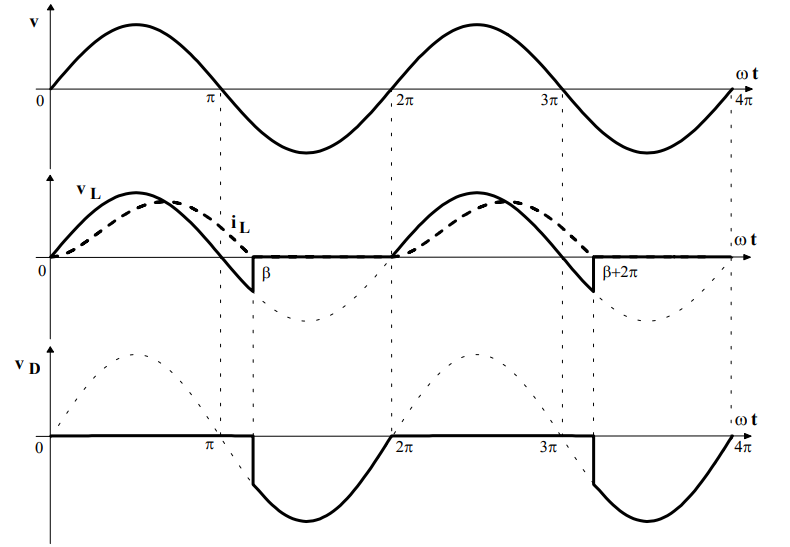
\includegraphics[width=0.6\textwidth]{imagens/FormasOndas.png}
\caption{Formas de onda das tensões e corrente no circuito do retificador de meia onda a diodo com carga indutiva.}\label{fig:FO}
\caption*{Fonte: EI I - Capitulo 2 - UNESP \protect\footnotemark}
\end{figure}

\footnotetext{Disponível em: <www2.sorocaba.unesp.br/professor/flavioasg/ei/cap2.pdf> Acesso em set. 2018.}

Nesse circuito, modelamos a corrente na carga $I_L$ pela equação \[
I_{L}(\omega{t}) = {\frac{\sqrt{2}V_o}{\sqrt{R^2 + X^2}}\sin{\left(\omega{t}-\phi\right)} - I_{1}\left(0\right)e^{-t/\tau}}
,\] onde $\phi = \arctan{\frac{X}{R}}$, $ {X} = \omega{L} $,  $\tau = \frac{L}{R}$.

Podemos dividir a corrente do circuito em dois componentes $I_L = i_1 + i_2$, de forma que
\begin{align*}
    i_{1}(\omega{t}) &= {\frac{\sqrt{2}V_o}{\sqrt{R^2 + X^2}}\sin{\left(\omega{t}-\phi\right)}}\\
	i_{2} &= I_{1}\left(0\right)e^{-t/\tau}
\end{align*}
A corrente $i_{2}$ pode ser entendida como a corrente do transitório, enquanto $i_{1}$ é a resposta em regime permanente da carga RL, conforme ilustrado na figura \ref{RMMOACRLI}.

Sabendo que $I_{1}(0) = {\frac{\sqrt{2}V_o}{\sqrt{R^2 + X^2}}}\sin{(-\phi)}$, obtêm-se a expressão \[
 I_{L}(\omega{t}) = {\frac{\sqrt{2}V_o}{\sqrt{R^2 + X^2}}[\sin{\left(\omega{t}-\phi\right)} - \sin{(-\phi)}e^{-t/\tau}}]
.\]

\begin{figure}[h]
\center
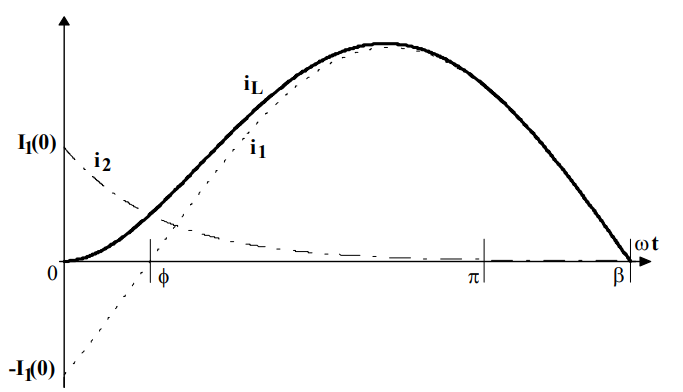
\includegraphics[width=0.6\textwidth]{imagens/correntedecarga.png}
\caption{Corrente de carga como no circuito da figura \ref{fig:RMMOACRL}.}\label{RMMOACRLI}
\caption*{Fonte: EI I - Capitulo 2 - UNESP $^1$}
\end{figure}

Quanto à tensão média aplicada na carga, é necessário modelar o valor do ângulo $\beta$. Para tal, observa-se que $i_{\omega}{t} = 0 $ quando ${\omega}{t} = {\beta}$.Dessa forma, substituindo ${\omega}{t} = {\beta}$ e sabendo que ${\omega}{\tau} = {\frac{\omega{L}}{R}} = {tg}{(\phi)}$, \[
\sin({\beta}-{\phi}) + \sin({\phi}){e^{-\beta/{ \tan({\tau})}}} = 0
.\] A relação entre $\beta$ e $\phi$ pode ser observada na figura \ref{fig:ACFA}. Portanto,
\begin{align*}
    V_{L,med} &= {\frac{1}{2\pi}{\int_{0}^{\beta}\sqrt{2}{V_o}{\sin({\omega}{t})}}d({\omega}{t})} \\
&\approx 0,225{V_o(1 - \cos({\beta}))}
.\end{align*}

\newpage
\begin{figure}[ht]
\center
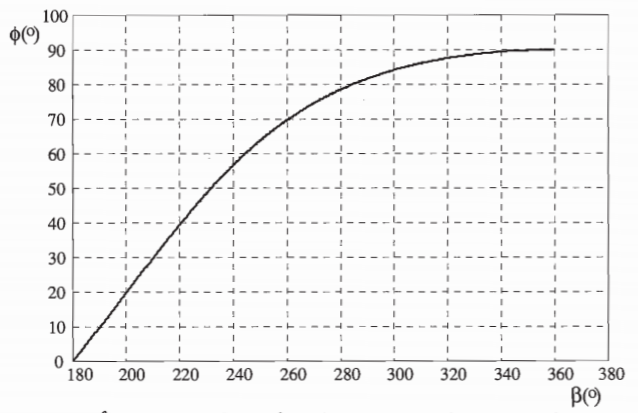
\includegraphics[scale=0.8]{imagens/grafico_variacao_beta_com_phi.PNG}
\caption{${\beta}$ em função de ${\phi}$.}\label{fig:ACFA}
\caption*{Fonte: Eletrônica de Potência (2006)}
\end{figure}

A partir dessa equação, vê-se que a tensão média na carga é inferior ao caso puramente resistivo. Além disso, como $V_{L,med} = 0 $ \[
I_{L,med} = \frac{0,225{V_o(1 - \cos({\beta}))}}{R}
.\] 

Uma forma de combater os efeitos da indutância no circuito é através de um diodo roda livre paralelo à carga. Dessa forma o circuito apresenta duas etapas de funcionamento. A primeira durante o semiciclo positivo da tensão de alimentação, na qual o diodo principal encontra-se polarizado e o diodo de roda livre está polarizado reversamente. A segunda durante o semiciclo negativo, na qual a corrente resultante da ação da indutância circula pelo diodo de roda livre, polarizado diretamente, enquanto o diodo principal polariza-se inversamente. A resposta desse circuito pode ser analisada através da figura \ref{fig:VIDRL}.

\begin{figure}[ht]
\center
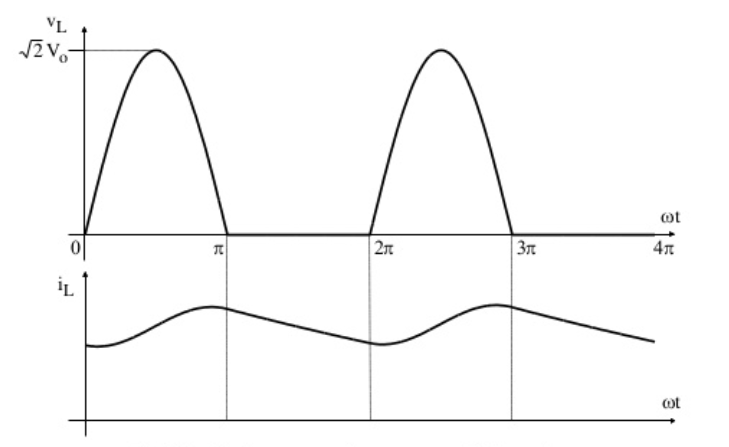
\includegraphics[scale=0.75]{imagens/VeIparaDRL.PNG}
\caption{Tensão e corrente na carga com componente indutivo no circuito com diodo de roda livre para condução contínua.}\label{fig:VIDRL}
\caption*{Fonte: Eletrônica de Potência (2006)}
\end{figure}

Para obter o modelo da corrente e da tensão na carga supõe-se que a estrutura encontra-se em regime permanente e em condução contínua. Pela série de Fourier para o sinal de entrada senoidal, podemos escrever \[
V_{L}(\omega{t}) = \frac{\sqrt{2}V_o}{\pi} + \frac{\sqrt{2}V_o}{2}{\sin({\omega}{t})} - {2}\frac{\sqrt{2}V_o}{\pi}[{\frac{\cos(2{\omega}{t)}}{1\cdot 3}}+{\frac{\cos(4{\omega}{t)}}{3\cdot 5}}+{\frac{\cos(6{\omega}{t)}}{5\cdot 7}}...] 
,\] ou seja, a tensão e a corrente médias na carga serão 
\begin{align*}
    V_{L,med} &= 0,45 V_o \\
    I_{L,med} &= \frac{0,45_o}{R}
.\end{align*}

Uma situação comum do uso do retificador é quando é alimentado por um transformador, que permite a adaptação da tensão da fonte à tensão de operação da carga e o isolamento entre a carga e a rede. O circuito nessa situação torna-se o da figura \ref{fig:TD}.

\begin{figure}[ht]
\center
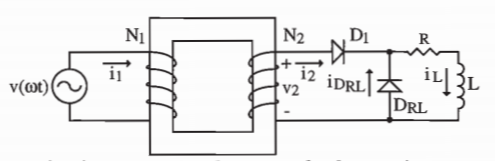
\includegraphics[scale=0.9]{imagens/trasformador_diodo.PNG}
\caption{Retificador monofásico de meia onda com diodo roda livre alimentado por um transformador.}\label{fig:TD}
\caption*{Fonte: Eletrônica de Potência (2006)}
\end{figure}

A figura \ref{fig:FdOTD} ilustra as formas de ondas para o circuito apresentado acima.

\begin{figure}[ht]
\center
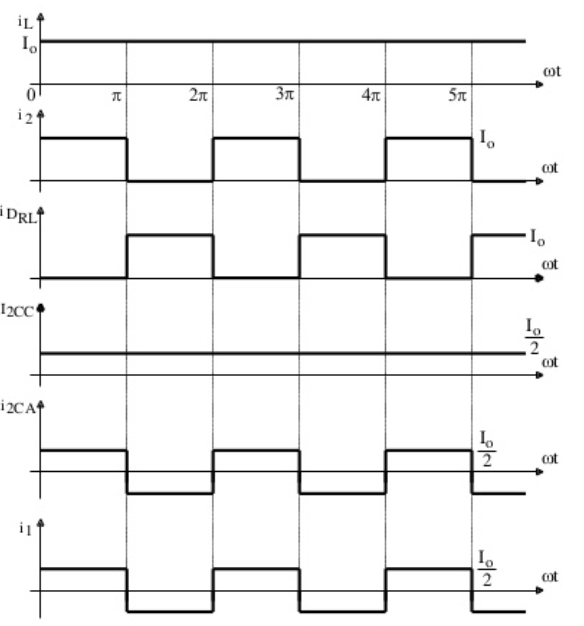
\includegraphics[scale=0.9]{imagens/formasdeOndaTransformador.PNG}
\caption{Formas de onda para o circuito da figura \ref{fig:TD}.}\label{fig:FdOTD}
\caption*{Fonte: Eletrônica de Potência (2006)}
\end{figure}

Sabemos que a potência e a tensão média da carga são dadas por
\begin{align*}
    P_{L} &= V_{L,med}\cdot I_{L,med} \\
    V_{L,med} &= 0,45 V_2
.\end{align*}

O uso mais comum para o retificador monofásico de meia onda é na alimentação da armadura de pequenos motores de corrente contínua, na alimentação de enrolamentos de excitação de máquinas elétricas, no carregamento de baterias e na alimentação de circuitos eletrônicos. 


 
\subsubsection{Retificadores monofásicos de onda completa com ponto médio}

Um circuito comumente utilizado para a implementação do retificador monofásico de ponto médio alimentado por um transformador pode ser observado na figura \ref{fig:RMOCDPM}. 

\begin{figure}[ht]
\center
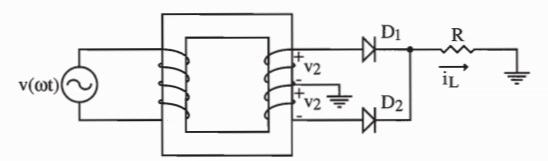
\includegraphics[scale=0.9]{imagens/ret_mono_ondaCompleta_cargaResistiva.PNG}
\caption{Retificador monofásico a diodo de onda completa com ponto médio, com carga puramente resistiva.}\label{fig:RMOCDPM}
\caption*{Fonte: Eletrônica de Potência (2006)}
\end{figure}

Pela análise desse circuito podemos notar que ele possui duas etapas de funcionamento relativas aos momentos de condução de cada um dos diodos. Ou seja, em cada semiciclo da fonte de alimentação, um dos diodos entra em condução. Como eles estão conectados de forma simétrica em relação ao ponto médio do enrolamento no secundário do transformador, a tensão aparente à carga em cada uma dessas etapas de funcionamento é idêntica. A figura \ref{fig:EFCR} demonstra essas etapas de funcionamento.

\begin{figure}[ht]
\center
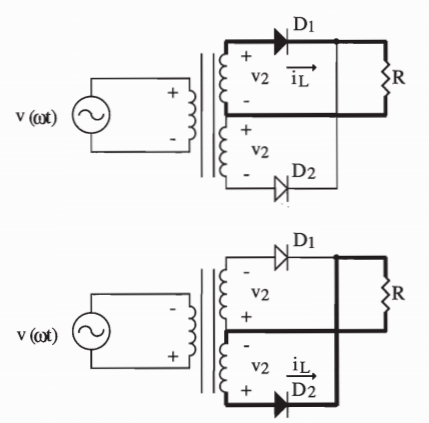
\includegraphics[scale=1.2]{imagens/etapas_funcio_ondaComp_pontoMedio.PNG}
\caption{Etapas de Funcionamento do circuito retificador de onda completa com ponto médio.}\label{fig:EFCR}
\caption*{Fonte: Eletrônica de Potência (2006)}
\end{figure}

O valor médio da tensão na carga pode ser modelado por
\begin{align*}
    V_{L,med} &= \frac{1}{\pi}{\int_{0}^{\pi}}{\sqrt{2}V_2{\sin(\omega{t})d(\omega{t})}} \\
	      &= 0,9 V_2 \\
    \implies I_{L,med} &= \frac{0,9 V_2}{R}
.\end{align*}

A corrente de pico na carga e nos diodos pode ser descrita por \[
I_{p} = \frac{\sqrt{2}V_2}{R}
.\] Dessa forma, a tensão de pico inversa dos diodos é \[
V_{Dp} = {2}\sqrt{2}V_2
.\] 

O valor médio da corrente em cada diodo é igual à metade do valor médio da corrente na carga, portanto \[
I_{D,med} = \frac{0,9 V_2}{2R}
.\] 

Os valor eficaz da corrente na carga é \[
I_{L,ef} = \frac{V_2}{R}
.\] 

Mesmo em um circuito em que a carga possui um componente indutivo, como na figura \ref{fig:ROCACI}, as etapas de funcionamento são as mesmas descritas para a carga resistiva pura.

\begin{figure}[ht]
\center
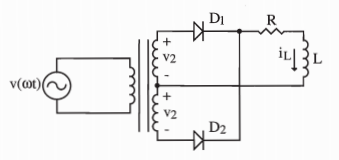
\includegraphics[scale=1.4]{imagens/CargaRL_ondaComple_pontoMedio.PNG}
\caption{Retificador de onda completa com ponto médio com uma carga com componente indutivo.}\label{fig:ROCACI}
\caption*{Fonte: Eletrônica de Potência (2006)}
\end{figure}

Para obter o equacionamento da corrente na carga novamente utiliza-se a série de Fourier, de forma que
\begin{align*}
    V_{L}(\omega{t}) &= \sqrt{2}V_2[{\frac{2}{\pi}-\frac{4}{3\pi}{\cos({2\omega}{t})}} - \frac{4}{15\pi}{\cos(4{\omega}{t})} - ...] \\
    I_{L}(\omega{t}) &= \sqrt{2}V_2[{\frac{2}{R\pi}-\frac{4}{3\pi{Z_2}}{\cos({2\omega}{t}-\phi_2)}} - \frac{4}{15\pi{Z_4}}{\cos(4{\omega}{t}-\phi_4)} - ...]
,\end{align*}
em que
\begin{align*}
Z_n &= \sqrt{R^2 + {n^2}{\omega}{L^2}} \text{, e} \\
\phi_n &= \tan^{-1}(\frac{n{\omega}{L}}{R})
.\end{align*}

Assim, obtém-se a corrente e tensão médias na carga modeladas por
\begin{align*}
    I_{L,med} &= \frac{2\sqrt{2}{V_2}}{\pi{R}} = \frac{0,9 V_2}{R} \\
    V_{L,med} &= 0,9 V_2
,\end{align*}
logo, \[
I_{D,med} = \frac{0,45 V_2}{R}
.\] 

O valor eficaz da corrente num diodo é \[
I_{D,ef} = 0,707{I_{L,med}}
.\] 

Dessa forma, vemos que a tensão e a corrente na carga segue como ilustrado na figura \ref{fig:TCCROCACI}.

\begin{figure}[ht]
\center
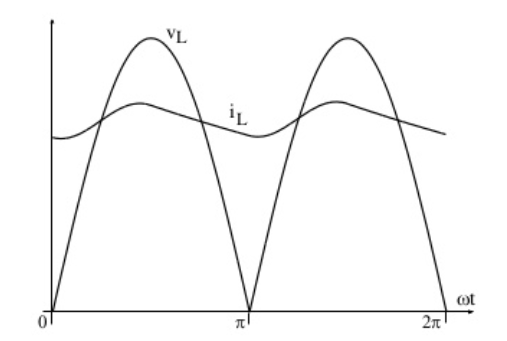
\includegraphics[scale=1.0]{imagens/tensaocorrentedecarga.PNG}
\caption{Tensão e corrente de carga para o circuito da figura \ref{fig:ROCACI}.}\label{fig:TCCROCACI}
\caption*{Fonte: Eletrônica de Potência (2006)}
\end{figure}

Para entender o comportamento da tensão e da corrente no transformador, podemos analisar o circuito entendendo a carga como uma fonte de corrente, como na figura \ref{fig:ESTOC}.

\begin{figure}[ht]
\center
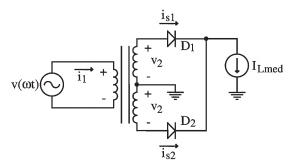
\includegraphics[scale=1.4]{imagens/estrutura_transf_onda_completa.PNG}
\caption{Circuito para o estudo do comportamento do transformador.}\label{fig:ESTOC}
\caption*{Fonte: Eletrônica de Potência (2006)}
\end{figure}

A corrente eficaz de um dos enrolamentos no secundário do transformador é
\begin{align*}
I_{sl,ef} = I_{s2l,ef} = \sqrt{ \frac{1}{2\pi}{\int_{0}^{\pi}}I_{L,med}^2{d(\omega{t})}} \\
I_{sl,ef} = I_{s2l,ef} \approx 0,707 I_{L,med} 
.\end{align*}


A potência aparente dissipada em um enrolamento do secundário é dada pela expressão \[
S_{s1} = V_{2,ef}I_{sl,ef}
.\] Como $V_{2ef} = \frac{V_{L,med}}{0,9}$, temos \[
S_{s1} \approx \frac{0,707 V_{L,med}I_{L,med}}{0,9} \approx 0,785 \,V_{L,med}I_{L,med}
.\] 

A potência aparente total no enrolamento secundário do transformador é \[
 S_{2} = S_{s1} + S_{s2}
,\] onde $S_{2} = 1,57 V_{L,med}I_{L,med}$
 Como a potência transferida à carga $P_{L} = V_{L,med}I_{L,med}$, \[
S_{2}= 1,57 P_{L}
.\] 

A tensão e a corrente no transformador se comportam conforme ilustrado na figura \ref{fig:FOC}.

\begin{figure}[ht]
\center
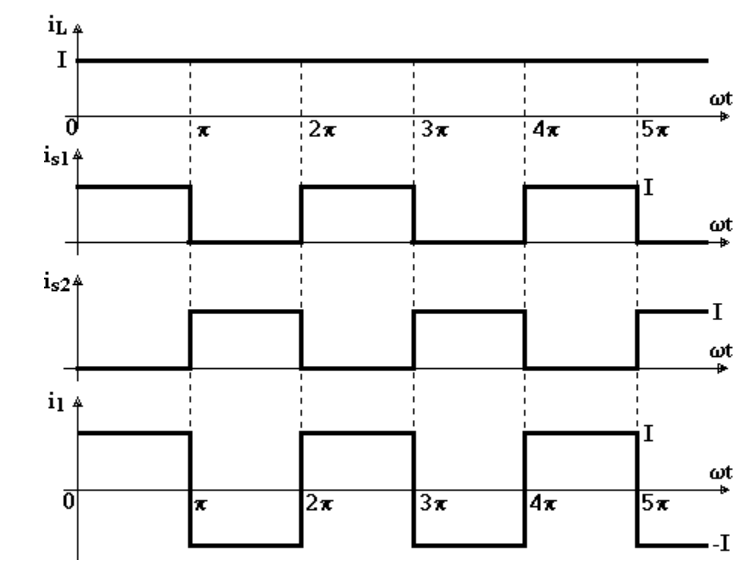
\includegraphics[scale=0.7]{imagens/FormaOndaCorrente.PNG}
\caption{Forma de onda das correntes.}\label{fig:FOC}
\caption*{Fonte: Eletrônica de Potência (2006)}
\end{figure}

Em relação ao retificador de meia onda, o retificador de onda completa se torna mais vantajoso por não resultar em uma corrente contínua no secundário do transformador, evitando a sua saturação. Além disso, a tensão média é duas vezes maior, além de resultar em uma corrente de carga com menor distorção harmônica.



\subsubsection{Retificadores monofásicos de onda completa em ponte}

Esta estrutura de retificador utiliza uma ponte de diodos para garantir um funcionamento similar ao do retificador com ponto médio, mas sem a necessidade de uma conexão intermediária no secundário do transformador, i.e., sem a necessidade de uma fonte simétrica. Tanto o circuito quanto as etapas de funcionamento são ilustradas na figura \ref{fig:CECT}.
 
\begin{figure}[ht]
    \center
    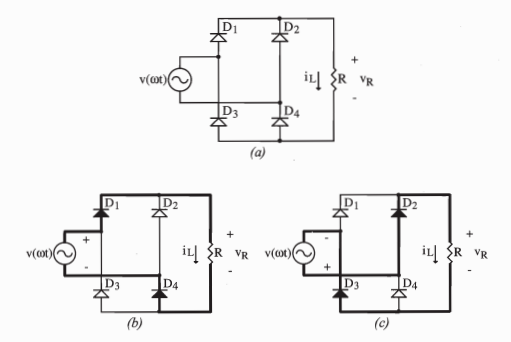
\includegraphics[scale=1]{imagens/Retif_mon_Ponte.PNG}
    \caption{(a) Circuito do retificador monofásico de onda completa em ponte com uma carga resistiva. (b) e (c) Etapas de funcionamento da ponte de diodos.}\label{fig:CECT}
    \caption*{Fonte: Eletrônica de Potência (2006)}
\end{figure}

A principal diferença é que, lidando com componentes não ideais, a presença de dois diodos em condução a todo momento implica no dobro da queda de tensão para a carga.

A tensão e a corrente aparentes à carga são idênticas as já demonstradas para o retificador de ponto médio. Seus valores médios são
\begin{align*}
    V_{L,med} &= 0,9V_o \\
    I_{L,med} &= \frac{0,9V_o}{R}
.\end{align*}

Novamente, as etapas de funcionamento apresentadas para a carga resistiva se mantém para uma carga indutiva. O comportamento também se mantém idêntico ao caso do ponto médio.

A presença de um transformador pode ser analisada de forma similar ao caso do retificador de meia onda, uma vez que o secundário não mais precisa ter uma conexão intermediária como no caso do retificador com ponto médio. Tal circuito é ilustrado na figura \ref{fig:RPAT}.

\begin{figure}[ht]
    \center
    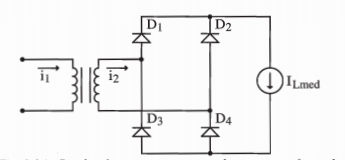
\includegraphics[scale=1]{imagens/RetPontTransf.PNG}
    \caption{Retificador em ponte alimentado por um transformador.}\label{fig:RPAT}
    \caption*{Fonte: Eletrônica de Potência (2006)}
\end{figure}

A corrente eficaz no secundário é 
\begin{align*}
    I_{2,ef} &= \sqrt{ \frac{1}{2\pi} \int_0^{2\pi} I_{L,med}^2 d(\omega{t}) } \\
	      &= I_{L,med}
,\end{align*}
enquanto a tensão é \[
V_{2,ef} = \frac{V_{L,med}}{0,9}
.\] 

Dessa forma, podemos determinar a potência aparente do transformador \[
    S_2 = V_{2,ef}{I_{2,ef}} = \frac{V_{L,med} {I_{L,med}}}{0,9}
,\] sendo $P_{L} = V_{L,med}I_{L,med}$, portanto \[
    S_2 = 1,11 P_L
.\] 

Vemos que o retificador em ponte aproveita melhor o enrolamento do secundário do transformador do que o retificador de ponto médio.

Esses retificadores normalmente são utilizados na alimentação de circuitos eletrônicos mais comuns (e.g., eletrodomésticos, computadores), no carregamento de baterias e na alimentação de enrolamentos de campo de máquinas elétricas. 



\subsubsection{Retificadores trifásicos com ponto médio}
 
Podemos estudar o comportamento desse tipo de retificador através do circuito da figura \ref{fig:RTDPM}, i.e., uma associação de três retificadores monofásicos de meia onda.  Note que esse retificador opera na alimentação em uma estrutura Y, ou seja, nas tensões de fase com acesso ao neutro.

\begin{figure}[ht]
    \center
    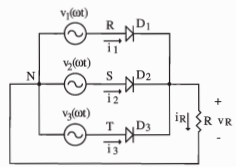
\includegraphics[scale=1.6]{imagens/RetTrifPontMed.PNG}
    \caption{Retificador trifásico a diodo com ponto médio.}\label{fig:RTDPM}
    \caption*{Fonte: Eletrônica de Potência (2006)}
\end{figure}

Nele, associamos um diodo a cada fase da alimentação, resultando nas formas de onda conforme ilustra a figura \ref{fig:FRTDPM}.

\begin{figure}[ht]
    \center
    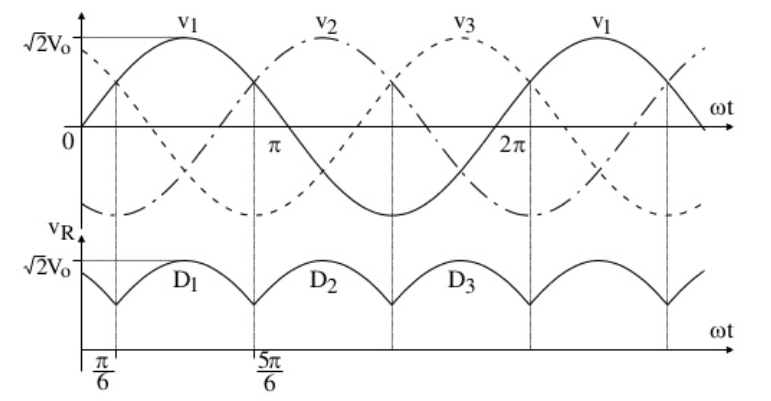
\includegraphics[scale=1]{imagens/FormasOndasRetTrifPont.PNG}
    \caption{Formas de onda para a figura \ref{fig:RTDPM}.}\label{fig:FRTDPM}
    \caption*{Fonte: Eletrônica de Potência (2006)}
\end{figure}

O valor da tensão média na carga é
\begin{align*}
V_{L,med} = \frac{3}{2\pi}{\int_{\frac{\pi}{6}}^{\frac{5\pi}{6}}}{\sqrt{2}{V_o}{\sin(\omega{t})}{d(\omega{t})}} \\
V_{L,med} = \frac{3{\sqrt{3}{\sqrt{2}}{V_o}}}{2\pi} \\
V_{L,med} = 1,17 V_o
.\end{align*}

Dessa forma, a corrente média na carga é \[
I_{L,med} = \frac{1,17 V_o}{R}
.\] 

A corrente médio nos diodos é \[
I_{D,med} = \frac{I_{L,med}}{3}
.\] 

O valor eficaz da corrente nos diodos pode ser calculado como
\begin{align*}
    I_{D,ef} &= \sqrt{\frac{1}{2\pi}{\int_{\frac{\pi}{6}}^{\frac{5\pi}{6}}}{[{\frac{\sqrt{2}{V_o}}{R}}{\sin(\omega{t})}}]^2{d(\omega{t})}} \\
	     &= 0,59{I_{Lmed}}
.\end{align*}

A expansão em série de Fourier da tensão na carga é
\begin{align*}
    V_{L}{(\omega{t})} &= 1,17{V_o} + \frac{2.1,17}{8}{V_o}{\sin(3\omega{t})} \\
    &= 1,17 V_o + 0,3V_o{\sin(3\omega{t})}
.\end{align*}
Dessa forma, a corrente na carga é \[
i_L(\omega{t}) = \frac{1,17 V_o}{R} + \frac{0,3 V_o}{\sqrt{R^2 + {9\omega^2}{L^2}}}{\sin(3\omega{t} - \phi_3)}
,\] onde \[{\phi_3} = \tan^{-1}{\frac{3\omega{t}}{R}}\]

O valor eficaz da corrente de carga pode ser calculado por \[
I_{L,ef} = \sqrt{(I_{L,med}^2 + I_{3,ef}^2)}
,\] onde $I_{L,med} = \frac{1,17 V_o}{R}$ e \[
I_{3,ef} = \frac{0,3 V_o}{\sqrt{2}{\sqrt{R^2 + 9\omega^2}{L^2}}}
.\] 
 
O valor eficaz da corrente em cada diodo (corrente eficaz de fase) é
\begin{align*}
I_{D,ef} &= \sqrt{\frac{1}{2\pi}{\int_{0}^{\frac{2\pi}{3}}}{(I_{L,med})^2}{d(\omega{t})}} \\
&= \frac{I_{L,med}}{\sqrt{3}}
.\end{align*}

O valor médio da corrente em cada diodo é definido através da corrente média da carga, i.e., \[
    I_{D,med} = \frac{I_{L,med}}{3}
.\]

Para o cálculo da tensão de pico sobre os diodos quando estes não estão conduzindo, utilizar-se-á o caso em que $D_2$ conduz a corrente da carga, como na figura \ref{fig:SEFCD}.

\begin{figure}[ht]
    \center
    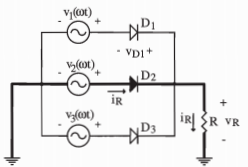
\includegraphics[scale=1.4]{imagens/SegEtapaFuncioD2.PNG}
    \caption{Segunda etapa de funcionamento do circuito.}\label{fig:SEFCD}
    \caption*{Fonte: Eletrônica de Potência (2006)}
\end{figure}

A tensão sobre o diodo $D_1$ pode ser determinada pela malha que contém $D_1$ e $D_2$, ou seja,
\begin{align*}
    \vec{V_1} + \vec{V}_{D_1} = \vec{V_2} + \vec{V_{D_2}} \\
    \implies \vec{V_{D1}} = \vec{V_2} - \vec{V_1}
.\end{align*}
Sendo $V_i$ a tensão eficaz da alimentação, então $V_{1,p} = \sqrt{2}{V_o}$ é o valor de pico da tensão de alimentação, logo \[
V_{D1p} = \sqrt{3}\sqrt{2}{V_o} \approx 2,45 V_o
.\] 



 
\subsubsection{Retificadores trifásicos de onda completa}

Para aproveitar todo o sinal fornecido pela alimentação, o retificador trifásico de onda completa utiliza uma ponte de Graetz, ou seja, de forma similar ao caso monofásico. Esse retificador aplica-se à alimentação em um arranjo $\Delta$, ou seja, sobre a tensão de linha, sem acesso ao neutro. Uma ilustração do circuito pode ser visto na figura \ref{fig:PGz}.

\begin{figure}[ht]
    \center
    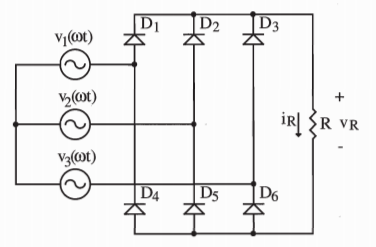
\includegraphics[scale=1.2]{imagens/PonteGraetz.PNG}
    \caption{Ponte de Graetz.}\label{fig:PGz}
    \caption*{Fonte: Eletrônica de Potência (2006)}
\end{figure}

A figura \ref{fig:FOASDRPM} mostra as formas de onda da saída.

\begin{figure}[ht]
    \center
    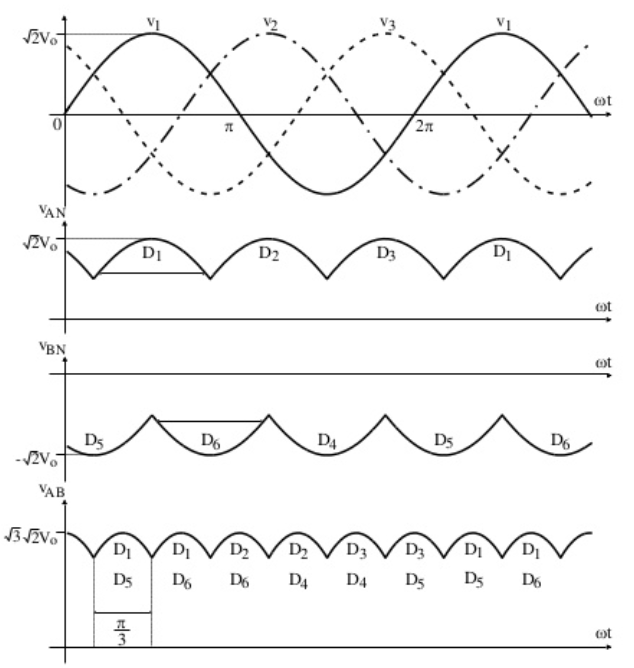
\includegraphics[scale=0.9]{imagens/FormasOndasDoisRet.PNG}
    \caption{Formas de onda da associação em série de dois retificadores de ponto médio.}\label{fig:FOASDRPM}
    \caption*{Fonte: Eletrônica de Potência (2006)}
\end{figure}

Veja que pode-se analisar a ponte de Graetz como uma associação em série de dois retificadores trifásicos de ponto médio. Além disso, vemos que os diodos entram em condução sempre em intervalos de 120 graus, logo, pela defasagem de 60 graus entre eles, sempre dois diodos estão em condução, um referente a cada semiciclo. Dessa forma, a frequência fundamental resultante é 6 vezes aquela da alimentação.

Calculando o valor médio da tensão de carga será considerado a figura .
A partir da figura \ref{fig:FOASDRPM}, podemos calcular a tensão média na carga
\begin{align*}
V_{L,med} &= \frac{3}{\pi}{\int_{-\frac{\pi}{6}}^{\frac{\pi}{6}}}{\sqrt{3}{\sqrt{2}}{V_o}}\cos(\omega{t}) \\
&= 2,34 V_o
,\end{align*} 
onde $V_o$ é o valor eficaz da tensão de alimentação.

No diodo, a corrente média \[
    I_{D,med} = \frac{I_{L,med}}{3}
\] e a corrente eficaz \[
    I_{D,ef} = \frac{I_{L,med}}{\sqrt{3}}
.\]

Um retificador trifásico com ponte de Graetz é utilizada extensivamente na indústria, onde a alimentação trifásica é mais comum, nos componentes que são projetados para utilizar corrente contínua, principalmente para altas potências (maiores que 10 KW).



\subsection{Retificadores a Tiristor}

A principal vantagem de utilizar o tiristor em relação ao diodo é em aplicações de eletrônica de potência em grande escala, uma vez que permitem o controle de grandes quantidades de energia. Isso o permite ser utilizado na conversão de energia. Dessa forma, eles possuem grande aplicação industrial no acionamento de motores CC, estações retificadoras na transmissão CC, no acionamento de trens, etc. 

Por meio da excitação do terminal de controle, é possível controlar a saturação das séries de junções P-N do tiristor, alterando o estado de bloqueio para condução. Os exemplos mais utilizados são os tiristores SCR, DIAC e TRIAC.

\subsubsection{Retificadores monofásicos de meia onda}

Esse segue o mesmo arranjo do retificador a diodo. Pode-se ver na figura \ref{ccr} um simples circuito do retificador monofásico de meia onda a tiristor para uma carga resistiva. 

\begin{figure}[h]
\center
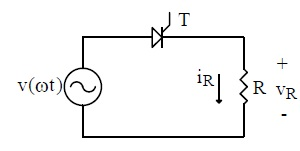
\includegraphics[scale=0.55]{imagens/circuito_carga_resistiva.jpg}
\caption{Circuito de um retificador a tiristor monofásico de meia onda com carga resistiva.}\label{ccr}
\caption*{Fonte: Eletônica de potência (2006)}
\end{figure}
  
Analisando as formas de onda na figura \ref{gcr} pode-se notar que até $\omega${t} = $\alpha$ a tensão na carga é nula, o que muda pela corrente de gatilho $i_{G}$. Assim, até o fim do semiciclo, a tensão de carga é igual à tensão da fonte. No semiciclo negativo, o tiristor encontra-se inversamente polarizado, i.e., não há tensão na carga.

\begin{figure}[h]
\center
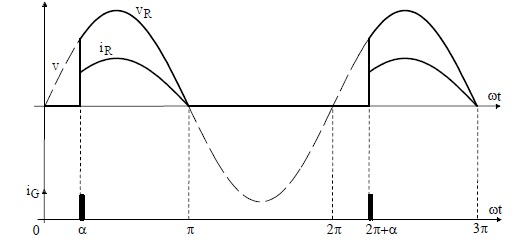
\includegraphics[scale=0.55]{imagens/grafico_carga_resistiva.jpg}
\caption{Formas de onda para retificador a tiristor monofásico de meia onda com carga resistiva.}\label{gcr}
\caption*{Fonte: Eletônica de potência (2006)}
\end{figure}

Portanto a tensão da fonte é calculada conforme a seguinte equação:
Assim, sendo $v(\omega t)=\sqrt{2}V_o\sin(\omega t)$ a tensão de alimentação, a tensão média na carga é
\begin{align*}
    V_{L,med} &= \frac{1}{2\pi}\int_\alpha^{\pi}\sqrt{2}V_o\sin(\omega t)d(\omega t) \\
&= \frac{\sqrt{2}V_o}{2\pi}[-cos(\omega t)]_\alpha^{\pi} \\
&\approx 0,225 V_o[1+\cos\alpha]
,\end{align*}
ou seja, a tensão média na carga é uma função do ângulo $\alpha$ de disparo do tiristor.

Dessa forma, a corrente média na carga é
\begin{align*}
    I_{L,med} &= \frac{V_{L,med}}{R} \\
    &\approx \frac{0,225 V_o}{R}(1+\cos\alpha)
.\end{align*}

A corrente eficaz na carga é
\begin{align*}
    I_{L,ef}&=\sqrt{\frac{1}{2\pi}\int_{\alpha}^{\pi}(\frac{\sqrt{2}V_o}{R})^{2}\sin^{2}(\omega t)d(\omega t)} \\
&=\sqrt{\frac{2V_o^{2}}{2\pi R^{2}}\int_{\alpha}^{\pi}\sin^2(\omega t)d(\omega t)} \\
&=\frac{V_o}{R}\sqrt{\frac{1}{\pi}\int_{\alpha}^{\pi}\sin^2(\omega t)d(\omega t)} \\
&=\frac{V_o}{R}\sqrt{\frac{1}{2}-\frac{\alpha}{2\pi}+\frac{\sin^2\alpha}{4\pi}}
.\end{align*}
A partir dela, pode-se determinar a potência por
\begin{align*}
    P_{R}&=RI_{L,ef}^{2} \\
	 &=\frac{V_{o}^{2}}{R}\left(   \frac{1}{2}-\frac{\alpha}{2\pi}+\frac{\sin^2\alpha}{4\pi}\right)
.\end{align*}

Caso a carga tenha um componente indutivo como no circuito da figura \ref{cti}, a característica indutiva gera um atraso na corrente, o que acarreta, tal qual no retificador a diodo, em um ângulo de bloqueio do diodo $\beta > \pi$, além do já estudado ângulo $\alpha$ para entrada em condução. As formas de onda da tensão e corrente na carga são ilustradas pela figura \ref{gti}.

\begin{figure}[h]
\center
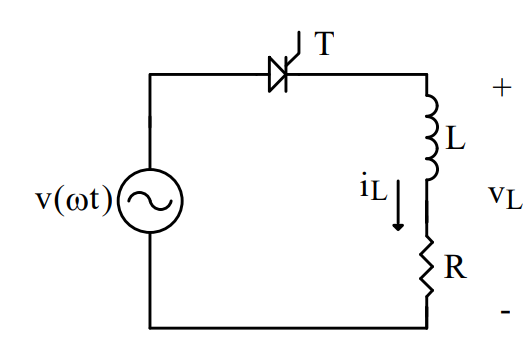
\includegraphics[scale=0.55]{imagens/circuito_tiristor_indutor.png}
\caption{Circuito de um retificador monofásico de meia onda a tiristor com carga indutiva.}\label{cti}
\caption*{Fonte: Eslaides aula 7 retificador a tiristor - Denizar Martins}
\end{figure}

\begin{figure}[h]
\center
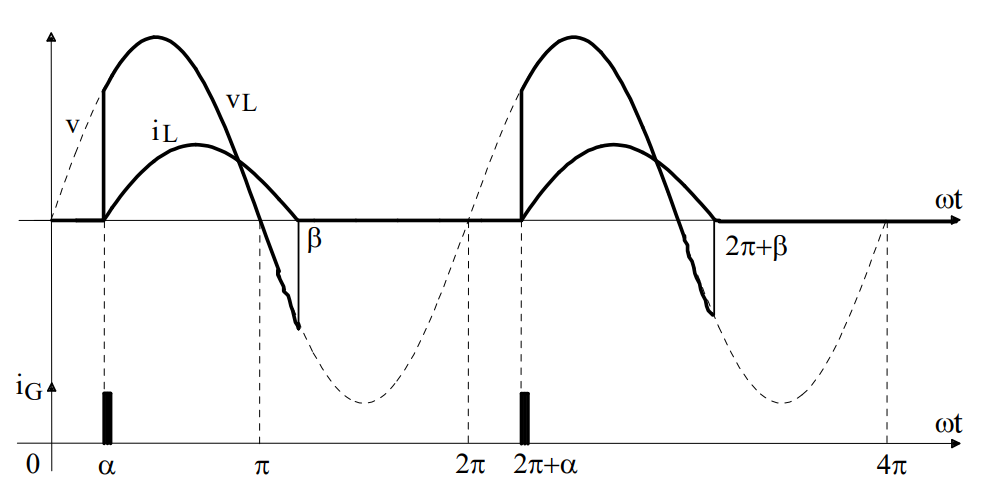
\includegraphics[scale=0.55]{imagens/grafico_tiristor_indutor.png}
\caption{Formas de onda de um retificador monofásico de meia onda a tiristor com carga indutiva.}\label{gti}
\caption*{Fonte: Eslaides aula 7 retificador a tiristor - Denizar Martins}
\end{figure}

Mais uma vez, sabe-se que, a partir do ângulo $\alpha$, a tensão na malha pode ser expressa através da corrente $i_L$ na carga, ou seja, \[
0 = Ri_{L}(wt) + L\frac{di_{L}(wt)}{dt} -v(wt)
,\] logo, \[
i_{L}(\omega{t}) = {\frac{\sqrt{2}V_o}{\sqrt{R^2 + X^2}}\sin{\left(\omega{t}-\phi\right)}e^{-t/\tau}}
,\] onde $\phi = \arctan{\frac{X}{R}}$, $ {X} = \omega{L} $ e $\tau = \frac{L}{R}$.

Podemos entender a corrente como a soma de dois componentes $i_L = i_1 + i_2$, sendo esses 
\begin{align*}
    i_{1}(\omega{t}) &= {\frac{\sqrt{2}V_o}{\sqrt{R^2 + X^2}}\sin{\left(\omega{t}-\phi\right)}} \\
    i_{2}(\omega{t}) &= {\frac{-\sqrt{2}V_o}{\sqrt{R^2 + X^2}}\sin{\left(\alpha-\phi\right)}e^{\frac{-t}{\tau}}}
.\end{align*}
Esses componentes representam, respectivamente, a corrente que circula em regime permanente e a corrente do transitório.

A tensão média na carga é
\begin{align*}
    V_{L,med} &= \frac{1}{2\pi}\int_\alpha^{\beta}\sqrt{2}V_o\sin(\omega t)d(\omega t) \\
&\approx 0,225 V_o[\cos\alpha - \cos\beta]
.\end{align*}
Fixando $V_{o}$ e $\alpha$, vemos que a tensão média na carga é função do ângulo $\beta$ que é uma função da constante de tempo da carga. Além disso, verificamos o resultado pela validade para a carga resistiva, em que $\beta = 1$, uma vez que as equações coincidem com as já discutidas.

A partir da tensão média, determinamos a corrente média na carga 
\begin{align*}
    I_{L,med} &= \frac{V_{L,med}}{R} \\
    &\approx \frac{0,225 V_o}{R}(\cos\alpha - \cos\beta)
.\end{align*}

O ângulo $\beta$ que controla o bloqueio do diodo pode ser determinado a partir de
\begin{align*}
    0 &= \frac{\sqrt{2}V_o}{\sqrt{R^2 + X^2}} \left[  \sin{\left(\beta-\phi\right)} -\sin{\left(\alpha-\phi\right)}e^{-\frac{\omega{R}}{\omega{L}}\left(  t -\frac{\alpha}{\omega}\right)} \right]  \\
    \implies 0 &= \sin(\beta - \phi) - \sin(\alpha - \phi)e^{\frac{R}{\omega{L}}(\beta - \alpha)}
,\end{align*}
que pode ser solucionada numericamente.

Com isso, determinamos a corrente eficaz na carga
\begin{align*}
    I_{L,ef}&=\sqrt{\frac{1}{2\pi}\int_{\alpha}^{\beta}i_{L}(\omega{t})^{2}d(\omega{t})} \\
&=\sqrt{\frac{1}{2\pi}\int_{\alpha}^{\beta}\left[\frac{\sqrt{2}V_{o}}{\sqrt{R^2 + X^2}}\left(  \sin(\omega{t}- \phi) - \sin(\alpha - \phi)e^{-\frac{R}{\omega{L}}(\omega{t}-\alpha)}\right)  ^{2}  \right] d(\omega{t})}
.\end{align*}

Para mitigar o problema da tensão negativa sobre a carga, pode-se adicionar ao circuito um diodo roda livre, resultando no circuito visível na figura \ref{cdc1}. Assim, também ilustrado na figura, o diodo permite a passagem da corrente induzida pelo indutor.

\begin{figure}[h]
\center
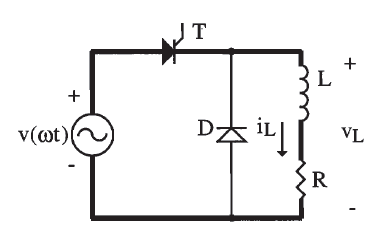
\includegraphics[width=0.45\textwidth]{imagens/circuito_diodo_circulacao1.png}
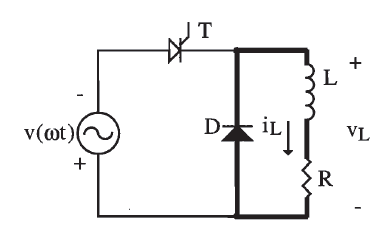
\includegraphics[width=0.45\textwidth]{imagens/circuito_diodo_circulacao2.png}
\caption{Circuito do retificador monofásico de meia onda a tiristor com diodo roda livre.}\label{cdc1}
\caption*{Fonte: Eletrônica de potência (2006)}
\end{figure}


A tensão e a corrente na carga estão representadas na figura \ref{gdc}. Vemos que a corrente na carga atinge seu valor máximo quando $\omega{t} = \omega{t}_{m}$, quando
\begin{align*}
    \frac{di_{L}(\omega{t})}{d(\omega{t})}&=0   \\
v_{1}(\omega{t})&=0
.\end{align*}

\begin{figure}[h]
\center
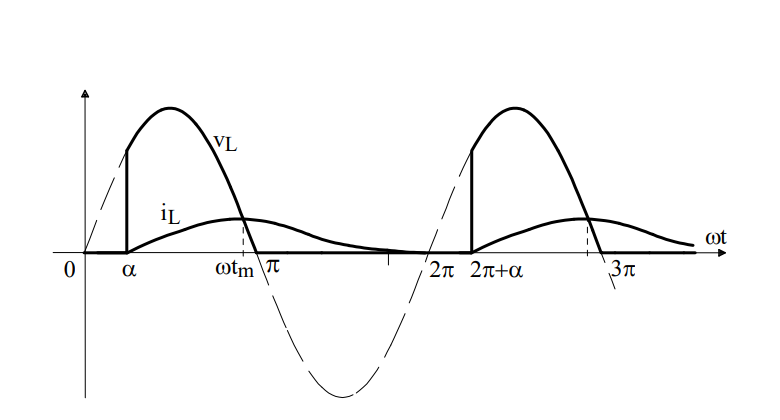
\includegraphics[scale=0.55]{imagens/formas_de_onda.png}
\caption{Tensão e corrente na carga do retificador monofásico de meia onda a tiristor com diodo de circulação.}\label{gdc}
\caption*{Fonte: Eletrônica de potência (2006)}
\end{figure}

A tensão média na carga é 
\begin{align*}
    V_{L,med} &= \frac{1}{2\pi}\int_{\alpha}^{\pi}\sqrt{2}V_{o}\sin(\omega{t}d(\omega{t}) \\
&= \frac{\sqrt{2}V_{o}}{2\pi}[-\cos(\omega{t})]_{\alpha}^{\pi} \\
&\approx 0,225V_{o}(1+\cos\alpha)
.\end{align*}
Veja que a tensão média não mais depende do ângulo $\beta$ e nem, portanto, da corrente de carga.

É evidente pela ilustração do seu comportamento que a corrente na carga se comporta de forma distinta em cada semiciclo da alimentação.

No semiciclo positivo, após $\alpha$, temos \[
i_{L1}(\omega{t}) = \frac{\sqrt{2}V_{o}}{\sqrt{R^2+X^2}}[\sin(\omega{t}-\phi)-\sin(\alpha-\phi)e^\frac{-t'}{\tau}]
,\] em que $t'=t-\frac{\alpha}{\omega}$.

No semiciclo negativo, até $\theta=\pi+5\omega \tau$,\[
i_{L1}(\omega(t)) = I_{1}e{^\frac{-t}{\tau}}
,\] onde $t''=t-\frac{\pi}{\omega}$.

Assim, \[
I_{1} = \frac{\sqrt{2}V_{o}}{\sqrt{R^2+X^2}}[\sin(\omega{t}-\phi)-\sin(\alpha-\phi)e^\frac{(\pi-\alpha)}{\omega\tau}]
,\] que nos permite refinar a nossa fórmula para a corrente de carga como \[
i_{L2}(\omega{t}) = \frac{\sqrt{2}V_{o}}{\sqrt{R^2+X^2}}[\sin(\omega{t}-\phi)-\sin(\alpha-\phi)e^\frac{(\pi-\alpha)}{\omega\tau}]e^\frac{(t-\pi/\omega)}{\tau}
.\] 



\subsubsection{Retificadores monofásicos de onda completa}

Há 3 possibilidades para aproveitar a onda completa com um retificador a tiristor. Primeiro, como ilustra a figura \ref{pc}, um retificador em ponte utilizando somente tiristores.

\begin{figure}[h]
\center
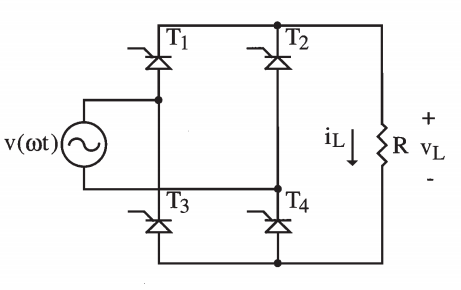
\includegraphics[scale=0.55]{imagens/ret_mono_comp_ponte.png}
\caption{Retificador de onda completa em ponte a tiristor.}\label{pc}
\caption*{Fonte: Eletrônica de potência (2006)}
\end{figure}

Essa é uma configuração relativamente redundante quanto ao controle, uma vez que não faz sentido o controle individual dos dois tiristores de cada par que compõe os possívei de entrar em condução a cada semiciclo. Dessa forma, surgem as configurações mistas da figura \ref{pma}, que associam tiristores e diodos em pares.

\begin{figure}[h]
\center
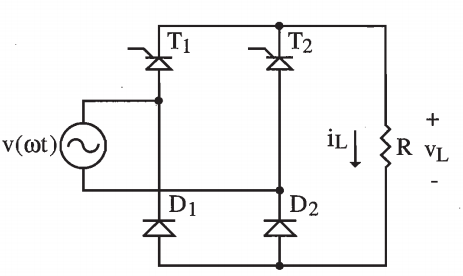
\includegraphics[width=0.45\textwidth]{imagens/ret_mono_comp_pontemista_a.png}
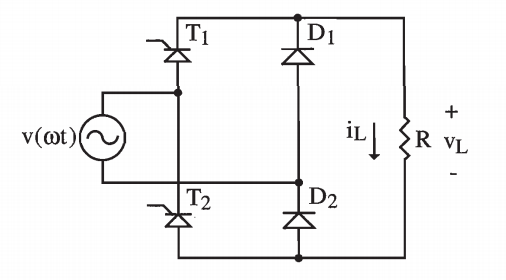
\includegraphics[width=0.45\textwidth]{imagens/ret_mono_comp_pontemista_b.png}
\caption{Retificador de onda completa com ponte mista A (esquerda) e B (direita).}\label{pma}
\caption*{Fonte: Eletrônica de potência (2006)}
\end{figure}

Por fim, há a configura com ponto médio tal qual a estudada para retificadores a diodo, como ilustra a figura \ref{pmed}. Novamente, destaca-se a necessidade de uma fonte simétrica como um secundário do transformador com uma conexão intermediária.

\begin{figure}[h]
\center
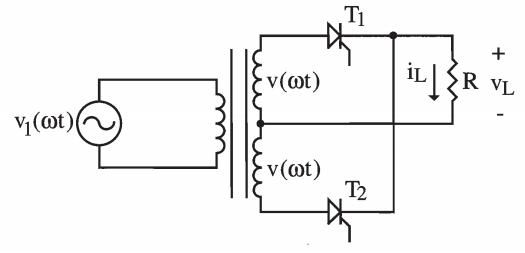
\includegraphics[scale=0.55]{imagens/ret_mono_comp_ponto_medio.png}
\caption{Retificador de onda completa a tiristor com ponto médio.}\label{pmed}
\caption*{Fonte: Eletrônica de potência (2006)}
\end{figure}

Ainda assim, o comportamento dessas implementações é o mesmo, como ilustra a figura \ref{gretr} no caso da carga resistiva, por isso serão estudados em conjunto.

\begin{figure}[h]
\center
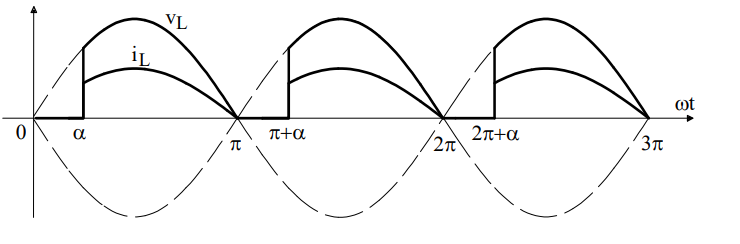
\includegraphics[scale=0.55]{imagens/grafico_ret_mono_comp.png}
\caption{Tensão e corrente em uma carga resistiva em um retificador de conda completa a tiristor.}\label{gretr}
\caption*{Fonte: Eletrônica de potência (2006)}
\end{figure}

Veja que até $\alpha$, quando um ou mais tiristores são ativados, a tensão na carga é nula. A partir desse momento, a tensão na carga (considerando o tiristor ideal) é tal qual a da alimentação. Assim, determinamos a tensão média
\begin{align*}
    V_{L,med} &= \frac{1}{\pi} \int_{0}^{\pi} \sqrt{2}V_{o}\sin(\omega{t})d(\omega{t})\\
&\approx 0,45V_{o}(1+\cos\alpha)
.\end{align*}
Verificamos que o resultado é condizente com a implementação a diodo uma vez que $\alpha=0$ implica na resposta já encontrada. Isso implica em uma relação entre a tensão média e o ângulo de disparo $\alpha$ como representada na figura \ref{gtmed}.

\begin{figure}[h]
\center
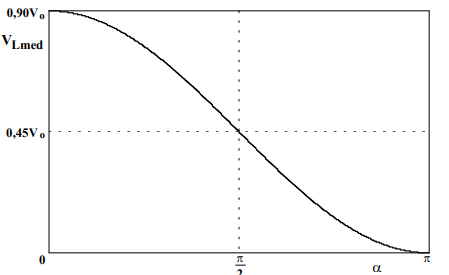
\includegraphics[scale=0.55]{imagens/ret_tensaomedia_resistivo.png}
\caption{Tensão média em função de $\alpha$ para carga resistiva no retificador de onda completa a tiristor.}\label{gtmed}
\caption*{Fonte:  EI I - Capitulo 3 - UNESP}
\end{figure}
\footnotetext{Disponível em: <www2.sorocaba.unesp.br/professor/flavioasg/ei/cap3.pdf> Acesso em set. 2018.}

Quando a carga possui componente indutivo é necessária a distinção entre as implementações. No caso do retificador totalmente controlado, tem-se o comportamento da tensão e da corrente na carga conforme ilustra a figura \ref{greti}. Aqui, utiliza-se:
\begin{description}
    \item[$\Delta$]  ângulo durante o qual a corrente de carga se mantém nula 
    \item[$\alpha$]  ângulo de disparo dos tiristores 
    \item[$\beta$] ângulo de extinção dos tiristores 
    \item[$\gamma$]  ângulo de condução
\end{description}

\begin{figure}[h]
\center
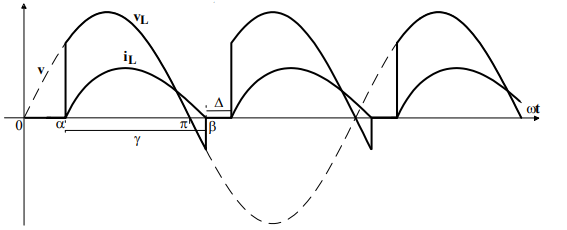
\includegraphics[scale=0.55]{imagens/grafico_ret_tensao_indutivo.png}
\caption{Tensão e corrente na carga com componente indutivo no retificador de onda completa a tiristor.}\label{greti}
\caption*{Fonte: Eletrônica de potência (2006)}
\end{figure}

Assim, a tensão média é
\begin{align*}
    V_{L,med} &= \frac{1}{\pi}\int_{0}^{\beta}\sqrt{2}V_{o}\sin(\omega{t})d(\omega{t}) \\
&\approx 0,45V_{o}(\cos\alpha - \cos\beta)
.\end{align*}

Já a corrente de carga pode ser determinada tal qual no retificador de meia onda a tiristor, ou seja, \[
i(\omega{t}) = \frac{\sqrt{2}V_{o}}{\sqrt{R^2+X^2}}[\sin(\omega{t}-\phi)-\sin(\alpha-\phi)e^\frac{-t'}{\tau}]
,\] onde $\phi = \arctan\frac{X}{R}$, $\tau = \frac{L}{R}$ e $t' =  t - \frac{\alpha}{\omega}$.

Veja que a condução é crítica se $\Delta = 0$ e, consequentemente, $\gamma = \pi$. A indutância crítica, que resulta na condução crítica, pode ser determinada sabendo-se que $i(\omega{t}) = 0$ quando $\beta = \pi + \alpha$, de forma que
\begin{align*}
 0 &= \sin(\pi+\alpha-\phi) - \sin(\alpha - \phi)e^{\frac{\pi}{\omega\tau}} \\
\omega\tau &= \frac{\omega{L}}{R} = \tan\phi \\
 \implies 0 &= \sin(\pi+\alpha-\phi) - \sin(\alpha - \phi)e^{\frac{\pi}{\tan\phi}}
.\end{align*}

Uma vez que essa igualdade só é válida para $\alpha=\phi$, pode-se substituir esse valor em $\omega\tau = \frac{\omega{L}}{R} = \tan\phi$ para determinar o valor da indutância crítica.

No caso de condução descontínua, $\omega{t}=\beta \implies i(\omega{t})=0$. Assim,
\begin{align*}
 0 &= \sin(\beta-\phi) - \sin(\alpha - \phi)e^{\frac{t'}{\tau}} \\
t' &= t - \frac{\alpha}{\omega} = \frac{\omega{t}}{\omega} - \frac{\alpha}{\omega} = \frac{\beta-\alpha}{\omega} \\
 \implies 0 &= \sin(\beta-\phi) - \sin(\alpha - \phi)e^{\frac{\beta-\alpha}{\tan\phi}}
.\end{align*}
De forma numérica, é possível determinar $\beta$ a partir de $\alpha$ e $\phi$.

Agora, podemos ver que o ângulo da tensão média, fixando-se $\alpha, \omega, V_{o}$ e L, depende apenas da resistência R da carga. Essa relação é ilustrada pela figura \ref{gretioc0}.

\begin{figure}[h]
\center
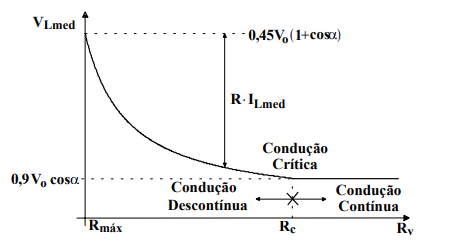
\includegraphics[scale=0.75]{imagens/grafico_ret_carga_indutivo.png}
\caption{Relação entre a tensão média e o componente resistivo da carga em um retificador de onda completa em ponte a tiristor.}\label{gretioc0}
\caption*{Fonte: EI I - Capitulo 3 - UNESP}
\end{figure}

Em condução descontínua, podemos modelar o retificador como uma fonte ideal em série com uma resistência variável pela corrente $I_{L,med}$, como ilustrado na figura \ref{cgretioc}.

\begin{figure}[h]
\center
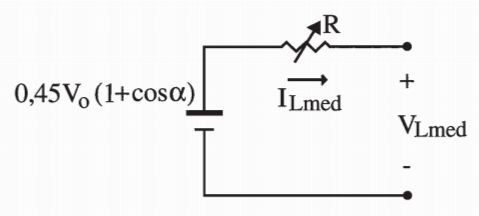
\includegraphics[scale=0.55]{imagens/circuito_equevalente.png}
\caption{Circuito equivalente de saída para o retificador de onda completa a tiristor.}\label{cgretioc}
\caption*{Fonte: Eletrônica de potência (2006)}
\end{figure}

Já no caso da condução contínua,
\begin{align*}
\beta &= \pi + \alpha \\
\implies V_{L,med} &= 0,45V_{o}(\cos\alpha - \cos\beta) \\
&= 0,45V_{o}[\cos\alpha - \cos(\pi+\alpha)] \\
&= 0,9V_{o}\cos\alpha
,\end{align*}
comportamento ilustrado na figura \ref{gretinv}.

\begin{figure}[h]
\center
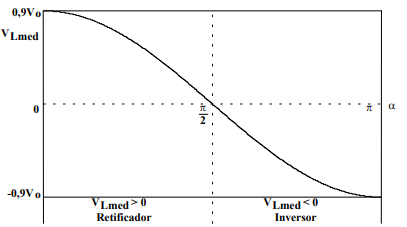
\includegraphics[scale=0.55]{imagens/grafico_ret_inversor.png}
\caption{Gráfico da tensão média para o retificador de onda completa com carga indutiva em condução contínua.}\label{gretinv}
\caption*{Fonte:  EI I - Capitulo 3 - UNESP}
\end{figure}

Uma vez que a corrente é sempre positiva, podemos determinar o fluxo de potência entre a fonte e a carga através da tensão média, ou seja, quando essa é negativa, o circuito se torna um retificador. Esse fenômeno, característico do circuito da figura \ref{cretoc}, está ilustrado na figura \ref{gretiocb}. Ressalta-se que esse inversor só funciona para corrente alternada.

\begin{figure}[h]
\center
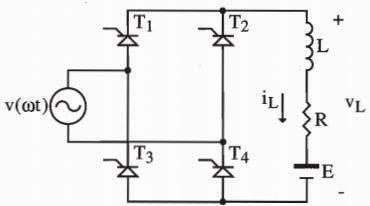
\includegraphics[scale=0.55]{imagens/circuito_ret_inversor.png}
\caption{Retificador de onda completa a tiristor atuando como inversor.}\label{cretoc}
\caption*{Fonte: Eletrônica de potência (2006)}
\end{figure}

\begin{figure}[h]
\center
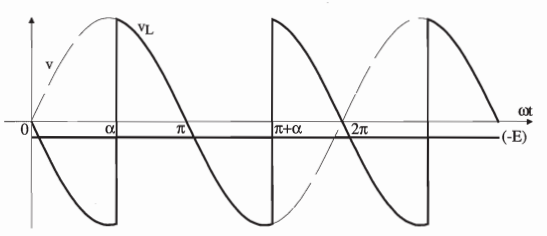
\includegraphics[scale=0.55]{imagens/grafico_conversor_inv.png}
\caption{Tensão da carga indutiva em um retificador de onda completa a tiristor atuando como inversor.}\label{gretiocb}
\caption*{Fonte: Eletrônica de potência (2006)}
\end{figure}

Tais retificadores totalmente controlados, que podem operar como inversores não autônomos, são bastante utilizados, por exemplo, em transmissão de energia elétrica a corrente contínua, tanto a retificação quanto a inversão, uma vez que podem ser feitas ambas por esse componente.

Já no caso do retificador com ponte mista, os diodos atuam, naturalmente como diodos de roda livre, como ilustra a figura \ref{epm}.

\begin{figure}[h]
\center
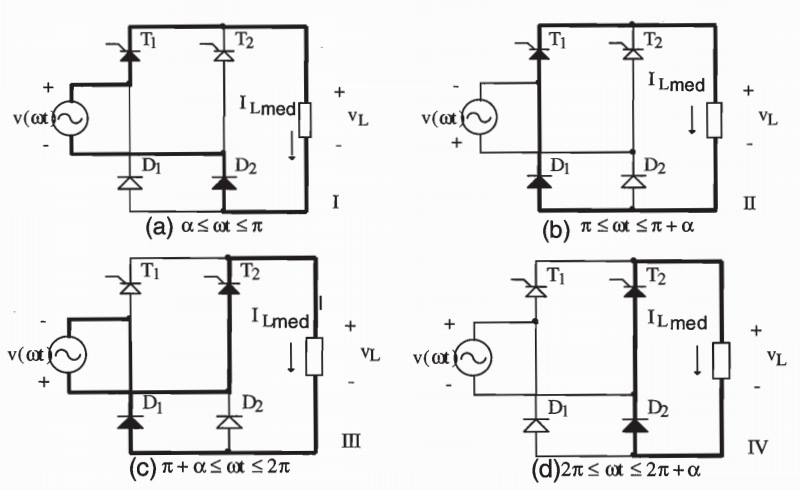
\includegraphics[scale=0.55]{imagens/etapas_ponte_mista.png}
\caption{Comportamento do retificador de onda completa com ponte mista com uma carga com componente indutivo.}\label{epm}
\caption*{Fonte: Eletrônica de potência (2006)}
\end{figure}

Da mesma forma, a tensão média é 
\begin{align*}
 V_{L,med} &= \frac{1}{\pi}\int_{\alpha}^{\pi}\sqrt{2}V_{o}\sin(\omega{t}d(\omega{t}) \\
 &= 0,45V_{o}[1+\cos(\alpha)]
.\end{align*}
Fica claro que essa configuração não funciona como um inversor.


 
\subsubsection{Retificadores trifásicos com ponto médio}

A configuração típica do retificador trifásico com ponto médio a tiristor pode ser observada na figura \ref{ctpm}. Define-se as tensões de alimentação (tensões de fase) igualmente defasadas, i.e.,
\begin{align*}
 V_{1}(\omega{t}) &= V_{o}\sin(\omega{t}) \\
 V_{2}(\omega{t}) &= V_{o}\sin(\omega{t}-120^0) \\
 V_{3}(\omega{t}) &= V_{o}\sin(\omega{t}+120^0)
.\end{align*}
 
 \begin{figure}[h]
\center
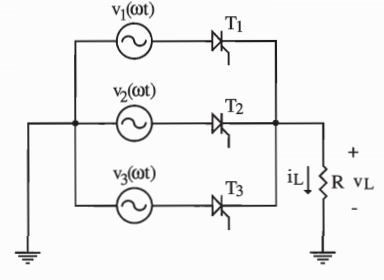
\includegraphics[scale=0.55]{imagens/circuito_trifasico_ponto_medio.png}
\caption{Circuito típico de um retificador trifásico de ponto médio a tiristor.}\label{ctpm}
\caption*{Fonte: Eletrônica de potência (2006)}
\end{figure}
 
 
A figura \ref{g1tm} ilustra a tensão na carga que possui somente componente resistivo. Veja que o ângulo de disparo $\alpha = 0$, gerando condução contínua. Na verdade, é fácil observar que isso é verdade para $\alpha < \frac{\pi}{6}$. Nesse caso, a tensão média pode ser calculada como
\begin{align*}
    V_{L,med} &= \frac{3}{2\pi}\int_{\frac{\pi}{6}+\alpha}^{\frac{5\pi}{6}+\alpha}\sqrt{2}V_{o}\sin(\omega{t})d(\omega{t}) \\
&= \frac{3\sqrt{2}V_{o}}{2\pi}[-\cos(\omega{t})]_{\pi/6+\alpha}^{5\pi/6+\alpha} \\
&= \frac{3\sqrt{2}\sqrt{3}V_{o}}{2\pi}\cos\alpha \\
&\approx 1,17\,V_{o}\cos\alpha
.\end{align*}
Veja que esse é o mesmo resultado do retificador a diodo, conforme esperado.

\begin{figure}[h]
\center
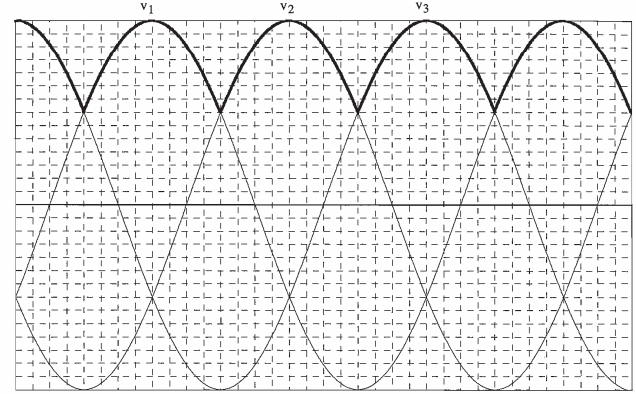
\includegraphics[scale=0.55]{imagens/grafico1_trifasico_ponto_medio_r.png}
\caption{Tensão na carga puramente resistiva para $\alpha = 0$ em um retificador trifásico de ponto médio a tiristor.}\label{g1tm} 
\caption*{Fonte: Eletrônica de potência (2006)}
\end{figure}

Para $\frac{5\pi}{6} > \alpha > \frac{\pi}{6}$, como ilustra a figura \ref{g2tm}, temos condução descontínua, ou seja, a tensão média se torna
\begin{align*}
    V_{L,med} &= \frac{3}{2\pi}\int_{\frac{\pi}{6}+\alpha}^{\pi}\sqrt{2}V_{o}\sin(\omega{t})d(\omega{t}) \\
&= \frac{3\sqrt{2}V_{o}}{2\pi}\left[-\cos\left(\omega{t}\right)\right]_{\frac{\pi}{6}+\alpha}^{\pi} \\
&= \frac{3\sqrt{2}V_{o}}{2\pi}\left[  1+\cos\left(  \frac{\pi}{6}+\alpha\right) \right]  \\
&\approx 0,675 V_{o}\left[  1+\cos\left(  \frac{\pi}{6}+\alpha \right) \right] 
.\end{align*}
Note que $\alpha = \frac{5\pi}{6} \implies V_{L,med} = 0$. O comportamento da tensão média em relação ao ângulo de disparo pode ser observado na figura \ref{g4tm}.

\begin{figure}[h]
\center
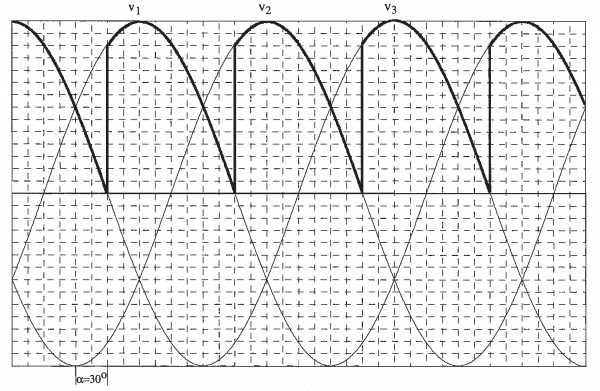
\includegraphics[width=0.45\textwidth]{imagens/grafico2_trifasico_ponto_medio_r.png}
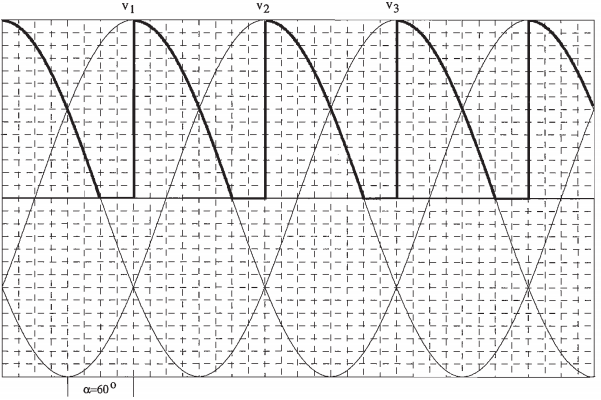
\includegraphics[width=0.45\textwidth]{imagens/grafico3_trifasico_ponto_medio_r.png}
\caption{Tensão na carga puramente resistiva para $\alpha = \frac{\pi}{6}$ (à esquerda) e $\alpha = \frac{\pi}{3}$ (à direita) em um retificador trifásico de ponto médio a tiristor.}\label{g2tm} 
\caption*{Fonte: Eletrônica de potência (2006)}
\end{figure}

\begin{figure}[h]
\center
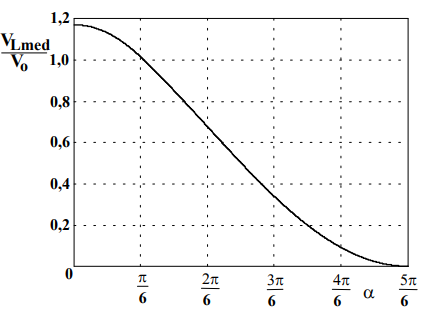
\includegraphics[scale=0.55]{imagens/grafico4_trifasico_ponto_medio_r.png}
\caption{$V_{L,med}$ em função de $\alpha$ de um retificador trifásico com ponto médio a tiristor para carga resistiva.} \label{g4tm} 
\caption*{Fonte: Eletrônica de potência (2006)}
\end{figure}

Para uma carga com componente indutivo de característica linar, a tensão média é dada por \[
V_{L,med} = 1,17V_{o}\cos\alpha
.\]
A figura \ref{g1tml} ilustra a tensão média em função de $\alpha$ para esse cenário.

\begin{figure}[h]
\center
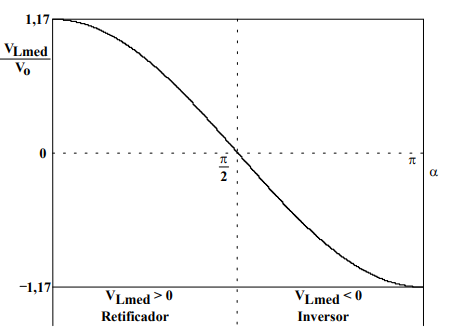
\includegraphics[scale=0.55]{imagens/grafico1_trifasico_ponto_medio_l.png}
\caption{$V_{L,med}$ em função de $\alpha$ em um retificador trifásico de ponto médio a tiristor com carga indutiva.} \label{g1tml} 
\caption*{Fonte: Eletrônica de potência (2006)}
\end{figure}

Veja que, como já visto anteriormente, essa estrutura pode operar tanto como retificador quanto como inversor. Esses dois modos de operação são visíveis na figura \ref{g2tml}.

\begin{figure}[h]
\center
\includegraphics[scale=0.55]{imagens/grafico2_trifasico_ponto_medio_l.png}
\includegraphics[scale=0.55]{imagens/grafico3_trifasico_ponto_medio_l.png}
\caption{Tensão média na carga com componente indutivo de um tiristor trifásico com ponto médio a tiristor para operação como retificador (à esquerda) e como inversor (à direita).} \label{g2tml} 
\caption*{Fonte: Eletrônica de potência (2006)}
\end{figure}


 
\subsubsection{Retificadores trifásicos de onda completa}

O retificador trifásico de onda completa utiliza uma ponte de Graetz, como já vimos. A figura \ref{ctcl} ilustra o circuito.

\begin{figure}[h]
\center
\includegraphics[scale=0.55]{imagens/circuito_trifasico_onda_completa.png}
\caption{Circuito do retificador trifásico de onda completa.} \label{ctcl} 
\caption*{Fonte: Eletrônica de potência (2006)}
\end{figure}

No caso da carga puramente resistiva, temos, primeiro, a situação do ângulo de disparo $\alpha = 0$, no qual é fácil ver que \[
V_{L,med} \approx 2,34 V_o
\] como já vimos para o caso equivalente implementado a diodo.

Já para $0<\alpha <\frac{\pi}{3}$, ainda há condução contínua e a tensão média na carga é 
\begin{align*}
    V_{L,med} &= \frac{6}{2\pi}\int_{\frac{\pi}{3}+\alpha}^{\frac{2\pi}{3}+\alpha}\sqrt{2}V_{OL}\sin(\omega{t})d(\omega{t})\\
	      &= \frac{6\sqrt{2}V_{OL}}{2\pi}\left[-\cos\left(\frac{2\pi}{3}+\alpha\right) + \cos\left(\frac{\pi}{3}+\alpha\right)\right] \\
    &= \frac{6\sqrt{2}V_{OL}}{2\pi}\cos\alpha\\
    &\approx 1,35V_{OL}\cos\alpha\\
    V_{OL} &= \sqrt{3}V_{o} \approx 1,73V_{o}\\
    \implies V_{L,med} &\approx 2,34V_{0}\cos\alpha
.\end{align*}

Para o caso da condução descontínua, i.e., $\frac{\pi}{3}<\alpha<\frac{2\pi}{3}$, a tensão média se torna
\begin{align*}
    V_{L,med} &= \frac{6}{2\pi}\int_{\frac{\pi}{3}+\alpha}^{\pi}\sqrt{2}V_{OL}\sin(\omega{t})d(\omega{t})\\
&\approx 2,34V_{o}\left[1 + \cos\left(\frac{\pi}{3}+\alpha \right)\right]
.\end{align*}

A relação entre a tensão média na carga e o ângulo de disparo pode ser observada na figura \ref{g1tcr}.

\begin{figure}[h]
\center
\includegraphics[scale=0.55]{imagens/grafico1_trifasico_onda_completa_r.png}
\caption{Tensão média na carga puramente resistiva de um retificador trifásico de onda completa a tiristor.} \label{g1tcr} 
\caption*{Fonte: Eletrônica de potência (2006)}
\end{figure}

Ambos os casos de condução são ilustrados na figura \ref{g1tcl}.

\begin{figure}[h]
\center
\includegraphics[scale=0.55]{imagens/grafico1_trifasico_onda_completa_l.png}
\caption{(a) Tensões de linha da rede. (b) Tensão na carga para $\alpha =0$. (c) Tensão na carga para $\alpha = \frac{\pi}{3}$. (d) Tensão na carga para $\alpha>\frac{\pi}{3}$ .} \label{g1tcl} 
\caption*{Fonte: Eletrônica de potência (2006)}
\end{figure}

Para uma carga com componente indutivo, a figura \ref{g2tcl} ilustra o comportamento da tensão na carga.

\begin{figure}[h]
\center
\includegraphics[width=0.45\textwidth]{imagens/grafico2_trifasico_onda_completa_l.png}
\includegraphics[width=0.45\textwidth]{imagens/grafico3_trifasico_onda_completa_l.png}
\caption{Tensão na carga com componente indutivo em um retificador trifásico de onda completa a tiristor.} \label{g2tcl} 
\caption*{Fonte: Eletrônica de potência (2006)}
\end{figure}

Nesse caso, a tensão média na carga é
\begin{align*}
    V_{L,med} &= \frac{3}{\pi}\int_{\frac{\pi}{3}+\alpha}^{\frac{2\pi}{3}+\alpha}\sqrt{2}V_{OL}\sin(\omega{t})d(\omega{t})\\
	      &= \frac{3\sqrt{2}V_{OL}}{\pi}\left[-\cos\left(\frac{2\pi}{3}+\alpha\right) +\cos\left(\frac{\pi}{3}+\alpha\right) \right] \\
&\approx 1,35V_{OL}\cos(\alpha)\\
&\approx 2,34V_{o}\cos(\alpha)
.\end{align*}

Dessa forma, é fácil ver que o circuito opera como um retificador para $0<\alpha<\frac{\pi}{2}$ e como um inversor não autônomo para $\frac{\pi}{2}<\alpha<\pi$.





\newpage

\section{Conversores}


Uma máquina de corrente contínua pode funcionar tanto como um gerador, convertendo energia mecânica em energia elétrica, quanto como um motor, convertendo energia elétrica em mecânica. Apesar de a energia elétrica ser comumente distribuída (no nível do consumidor) em corrente alternada, os motores de corrente contínua possuem grande participação na indústrias, uma vez que permitem facilmente a variação de velocidade, por exemplo, de uma esteira ou um comboio. 

Por outro lado, componentes eletrônicos de tensão alternada, cada vez mais acessíveis, são capazes de controlar a velocidade de motores assíncronos da mesma forma, logo, pelo seu melhor custo benefício, eles vêm substituindo os motores de corrente contínua na maior parte das aplicações. De toda forma, o estudo dos motores de corrente contínua é fundamental pois introduz os conceitos básicos do funcionamento de máquinas elétricas. A figura \ref{fig:MCC} mostra esquematicamente uma máquina de corrente contínua elementar.

\begin{figure}[ht!]
\center
\includegraphics[scale=0.66]{imagens/maquina_cc.png}
\caption{\label{fig:MCC}Máquina de corrente contínua elementar.}
\caption*{Fonte: Máquinas de corrente contínua \protect\footnotemark}
\end{figure}

\footnotetext{Disponível em: <http://www.gsep.ene.unb.br/osem/ivan/Conversao> Acesso em out. 2018.}



\subsection{Conversores CC-CC}

% 
Também conhecido como abaixador de tensão, a principal característica dos conversores buck é o controle da corrente na saída, conforme ilustra a figura \ref{cb}.

\begin{figure}[h]
\center
\includegraphics[scale=0.55]{imagens/circuito_buck.png}
\caption{Estrutura do conversor Buck.}\label{cb} 
\caption*{Fonte: Introdução aos conversores CC-CC (2001)}
\end{figure}
 
O seu funcionamento pode ser  descrito em duas etapas. Primeiro, com a chave $S$ em condução, i.e., no período $D \cdot T_s$, a fonte $V_i$ energiza o circuito RLC. No momento em que a chave $S$ abre, no período $\left( 1-D \right) T_s$, o circuito garante inércia da corrente sobre a saída.

Sabendo que a tensão média sobre o atuador, idealmente, é nula, podemos determinar 
\begin{align*}
    V_{o} &= V_{ab,med} =  \frac{1}{T_{s}}\int_{o}^{DT_{s}}V_{i}dt\\
	  &\implies \frac{V_{o}}{V_{i}} = D
.\end{align*} Ou seja, novamente temos uma relação linear entre a razão cíclica e o ganho estático.

A figura \ref{g3b} ilustra o comportamento da tensão e da corrente nos diversos componentes da carga do conversor buck.

\begin{figure}[h]
\center
\includegraphics[scale=0.55]{imagens/grafico3_buck.png}
\caption{Formas de onda do conversor Buck.}\label{g3b} 
\caption*{Fonte: Introdução aos conversores CC-CC (2001)}
\end{figure}

De forma similar ao que foi visto nos retificadores, o conversor buck também pode operar em condução contínua, descontínua ou crítica, quando encontra-se na iminência de trocar seu modo de operação.

De modo geral, o conversor Buck está limitado à magnitude da tensão da entrada, mas não tem grande impacto sobre a corrente da saída, i.e., não a distorce muito, ainda que chaveie sempre a corrente fornecida pela alimentação.


% 
% O maior diferencial do conversor Boost é a capacidade de elevar a tensão a partir da corrente na entrada. A figura \ref{cboost} ilustra o circuito simplificado de um conversor Boost.

\begin{figure}[h]
\center
\includegraphics[scale=0.55]{imagens/circuito_boost.png}
\caption{Circuito simplificado do conversor Boost.}\label{cboost} 
\caption*{Fonte: Introdução aos conversores CC-CC (2001)}
\end{figure}

Durante a etapa de condução, com a chave $S$ fechada, o indutor $L$ é magnetizado pela alimentação. Nota-se que a chave age como um curto para a saída, que só é alimentada pelo capacitor $C_o$ uma vez que há o diodo $D$ impedindo que esse seja curto-circuitado pela chave. Quando a chave abre, o indutor e a fonte fornecem energia à saída e ao capacitor, dessa forma, elevando a tensão aparente na saída. O comportamento da tensão no indutor pode ser visto, de forma simplificada, na figura \ref{g1bo}.

\begin{figure}[h]
\center
\includegraphics[scale=0.55]{imagens/grafico1_boost.png}
\caption{Comportamento da tensão no indutor de um conversor Boost.}\label{g1bo} 
\caption*{Fonte: Introdução aos conversores CC-CC (2001)}
\end{figure}

Assumindo, com idealidades, que a tensão média sobre o indutor é nula, temos \[
V_o = \frac{1}{T_{s}}\int_{o}^{DT_{s}}V_{i}dt =  \frac{1}{T_{s}}\int_{o}^{(1-D)T_{s}}(V_{o} - V_{i})dt
\] \[
\implies \frac{V{o}}{V{i}} = \frac{1}{1-D}
.\]

A relação entre a razão cíclica e o ganho estático pode ser vista na figura \ref{g2bo}.

\begin{figure}[h]
\center
\includegraphics[scale=0.55]{imagens/grafico2_boost.png}
\caption{Relação entre o ganho estático e a razão cíclica em um conversor Boost.}\label{g2bo} 
\caption*{Fonte: Introdução aos conversores CC-CC (2001)}
\end{figure}

O comportamento da tensão e da corrente nos componentes do conversor Boost é ilustrada na figura \ref{g3bo}.

\begin{figure}[h]
\center
\includegraphics[scale=0.55]{imagens/grafico3_boost.png}
\caption{Tensão e corrente nos componentes do conversor Boost.}\label{g3bo} 
\caption*{Fonte: Introdução aos conversores CC-CC (2001)}
\end{figure}

As principais características do conversor Boost são sua capacidade de aumentar a tensão da saída, apesar de fornecer corrente de forma descontínua, e baixa distorção da corrente consumida da alimentação.


% 
% Resultado da combinação dos dois conversores que dão nome a este, o conversor Buck-Boost consegue elevar e abaixar a tensão. A figura \ref{cbobu} ilustra um circuito simplificado para esse conversor.

\begin{figure}[h]
\center
\includegraphics[scale=0.55]{imagens/circuito_buck_boost.png}
\caption{Circuito do conversor Buck-Boost.}\label{cbobu} 
\caption*{Fonte: Introdução aos conversores CC-CC (2001)}
\end{figure}

Durante a etapa de condução da chave $S$, a fonte fornece energia para o indutor $L$, enquanto o capacitor $C_o$ descarrega sobre o resistor $R_o$. Após a abertura da chave $S$, o indutor alimenta tanto o capacitor quanto a resistência, mas de forma invertida à fonte. A figura \ref{g1bobu} ilustra a tensão no indutor $L$.

\begin{figure}[h]
\center
\includegraphics[scale=0.55]{imagens/grafico1_buck_boost.png}
\caption{Comportamento da tensão no indutor $L$ de um conversor Buck-Boost.}\label{g1bobu} 
\caption*{Fonte: Introdução aos conversores CC-CC (2001)}
\end{figure}

Considerando a tensão média no indutor nula, segue que \[
    \frac{1}{T_{s}}\int_{o}^{DT_{s}}V_{i}dt =  \frac{1}{T_{s}}\int_{o}^{(1-D)T_{s}}(V_{o} - V_{i})dt
\] \[
\implies\frac{V{o}}{V{i}} = \frac{D}{1-D}
.\] Logo, é fácil ver que o conversor pode tanto abaixar quanto elevar a tensão de forma contínua a partir da razão cíclica. A figura \ref{g2bobu} ilustra essa relação.

\begin{figure}[h]
\center
\includegraphics[scale=0.55]{imagens/grafico2_buck_boost.png}
\caption{Relação entre o ganho estático de um conversor Buck-Boost e a razão cíclica do chaveamento.}\label{g2bobu} 
\caption*{Fonte: Introdução aos conversores CC-CC (2001)}
\end{figure}

O comportamento da tensão e da corrente nos diversos componentes desse conversor está ilustrado na figura \ref{g2bobu}.

\begin{figure}[h]
\center
\includegraphics[scale=0.55]{imagens/grafico3_buck_boost.png}
\caption{Comportamento da tensão e da corrente nos diversos componentes de um conversor Buck-Boost.}\label{g3bobu} 
\caption*{Fonte: Introdução aos conversores CC-CC (2001)}
\end{figure}

Dessa forma, o conversor Buck-Boost fornece uma implementação que abaixa e eleva a tensão de forma contínua, mas distorce a corrente tanto para a alimentação quanto para a carga.


% 
\subsection{Conversores CC-CA}
% 
% Dois arranjos serão estudados para o inversor monofásico: em semi-ponte e em ponte completa. Ambos podem ser observados na figura \ref{c1im}.

\begin{figure}[h]
\center
\includegraphics[scale=0.55]{imagens/circuito1_inversor_mono.png}
\includegraphics[scale=0.55]{imagens/circuito2_inversor_mono.png}
\caption{Circuitos de um inversor monofásico em semi-ponte. À esquerda, em semi-ponte;  direita em ponte completa.}\label{c1im} 
\caption*{Fonte: Apostila de eletrônica de potência (2015)}
\end{figure}

No caso da implementação em semi-ponte, através do chaveamento dos transistores Q1 e Q2 pode-se controlar a tensão observada pela carga. A figura \ref{g1im} ilustra esse comportamento. Não é difícil ver que se o controle de Q2 é replicado em Q3 e o de Q1 em Q4, temos o mesmo resultado, para a carga, no caso da implementação em ponte completa mas com amplitude dobrada. Nota-se que a tensão percebida pela carga é uma onda quadrada, mas simétrica e com frequência constante, desde que a frequência de chaveamento o seja.

\begin{figure}[h]
\center
\includegraphics[scale=0.55]{imagens/grafico1_inversor_mono.png}
\caption{Tensão sobre a carga de um inversor monofásico em semi-ponte e correntes de acionamento dos transístores Q1 e Q2.}\label{g1im} 
\caption*{Fonte: Apostila de eletrônica de potência (2015)}
\end{figure}

Podemos, então, modelar a tensão de saída do inversor através da expansão em série de Fourier da onda quadrada gerada, i.e., \[
    v_{o} = \sum_{k=1}^{\infty}\frac{4A}{\left( 2k +1 \right) \pi}\sin{\left( 2k+1 \right) \omega{t}} 
,\] onde $A$ é a amplitude da tensão de saída (portanto $A = \frac{V}{2}$ para o inversor em semi-ponte e $A = V$ para o inversor em ponte completa), $\omega = 2\pi f$ é a frequência da tensão de saída.

Caso a carga seja puramente resistiva é evidente que a corrente possuirá o mesmo comportamento da tensão. No caso de uma carga com componente indutivo, a corrente na carga torna-se \[
    i_{o} = \sum_{k=1}^{\infty}\frac{4A}{\left( 2k+1 \right) \pi{|Z_{k}|}}\sin(\left( 2k+1 \right)\omega{t} - \phi_{k})
,\] onde $\tau = \frac{L}{R}$, $|Z_k| = \sqrt{R^{2} + (\left( 2k+1 \right) \omega{L})^2}$ e \[
\phi_{k} = \tan^{-1} \frac{\left( 2k+1 \right) \omega{L}}{R}
.\] 

Também pode-se escrever a corrente em função da amplitude $A$, de forma \[
i_o = \begin{cases}
    \frac{A}{R}(1-e^{-t/\tau}) &, t \in [0,\frac{T}{2}) \\
    \frac{-A}{R}(1-e^{-(t-\frac{T}{2})/\tau}) + I_{max}e^{-(t-\frac{T}{2})/\tau} &, t \in [\frac{T}{2},T)
\end{cases}
,\] onde: \[
    I_{MAX} = \frac{A}{R} \left(  \frac{1-e^{-\frac{T}{2\tau}}}{1+e^{-\frac{T}{2\tau}}}\right) 
.\]

Caso seja uma carga com componente capacitivo, a corrente pode ser descrita por \[
i_o = \begin{cases}
    I_{MAX}e^{-t/\tau} &, t \in \left[0,\frac{T}{2}\right) \\
    I_{MAX}e^{-(t-\frac{T}{2})/\tau} &, t \in \left[\frac{T}{2}, T\right)
\end{cases}
\] e a tensão \[
i_o = \begin{cases}
    A(1-e^{-t/\tau}) - V_{CO}e^{-t/\tau} &, t \in \left[0,\frac{T}{2}\right) \\
    A(1-e^{-(t-\frac{T}{2})/\tau}) + V_{C0}e^{-(t-\frac{T}{2})/\tau} &, t \in \left[\frac{T}{2}, T\right)
\end{cases}
,\] onde \[
    V_{C0} = A\frac{1-e^{-\frac{T}{2\tau}}}{1+e^{-\frac{T}{2\tau}}}
\] e \[
    I_{MAX} = \frac{A + V_{co}}{R}
.\]

A figura \ref{g3im} ilustra o comportamento da tensão e da corrente para ambas as cargas não lineares.

\begin{figure}[h]
\center
\includegraphics[scale=0.55]{imagens/grafico3_inversor_mono.png}
\includegraphics[scale=0.55]{imagens/grafico4_inversor_mono.png}
\caption{Corrente e tensão na carga de um inversor monofásico. À esquerda, carga RL; à direita, carga RC.}\label{g3im} 
\caption*{Fonte: Apostila de eletrônica de potência (2015)}
\end{figure}


% 
% 
O circuito característico de um inversor trifásico pode ser ilustrado como na figura \ref{c1it}.

\begin{figure}[h]
\center
\includegraphics[scale=0.55]{imagens/circuito1_inversor_tri.png}
\caption{Estrutura básica de um inversor trifásico}\label{c1it} 
\caption*{Fonte: Apostila de eletrônica de potência (2015)}
\end{figure}

Serão estudadas duas formas de comutação simples para esse tipo de inversor. A primeira, chamada de comutação seis-pulsos 180º, consiste em acionar cada um dos 6 transistores durante meio ciclo (daí os 180º) igualmente espaçados. O acionamento dos transistores encontra-se ilustrado na figura \ref{g1it}, junto do resultado para a carga em termos de tensão de fase e linha. Veja que a tensão de linha (eficaz) nesse modo de operação é \[
V_R = \sqrt{\frac{2}{3}} V
.\] 

\begin{figure}[h]
\center
\includegraphics[width=0.32\textwidth]{imagens/grafico1_inversor_tri.png}
\includegraphics[width=0.32\textwidth]{imagens/grafico2_inversor_tri.png}
\includegraphics[width=0.32\textwidth]{imagens/grafico3_inversor_tri.png}
\caption{Acionamento dos transistores (à esquerda) da ponte inversora trifásica em operação seis pulsos 180º, assim como a tensão de fase (ao centro) e de linha (à direita) para a carga.}\label{g1it} 
\caption*{Fonte: Apostila de eletrônica de potência (2015)}
\end{figure}

Já o modo de comutação seis-pulsos 120º modifica o período de ativação de cada transistor para $\frac{2}{3}$ do período desejado, gerando intervalos de tensão não determinada, como pode ser visto na figura \ref{g4it}, estando os transistores em estado de alta impedância.
 
\begin{figure}[h]
\center
\includegraphics[width=0.32\textwidth]{imagens/grafico4_inversor_tri.png}
\includegraphics[width=0.32\textwidth]{imagens/grafico5_inversor_tri.png}
\includegraphics[width=0.32\textwidth]{imagens/grafico6_inversor_tri.png}
\caption{Acionamento dos transistores (à esquerda) da ponte inversora trifásica em operação seis pulsos 120º, assim como a tensão de fase (ao centro) e de linha (à direita) para a carga. Regiões sólidas representam um valor não determinado pelo inversor.}\label{g4it} 
\caption*{Fonte: Apostila de eletrônica de potência (2015)}
\end{figure}

Caso a carga seja puramente resistiva, a tensão aparente para essa será como ilustrado na figura \ref{g7it}. A tensão de linha (eficaz), então, torna-se \[
V_R = \frac{\sqrt{2} }{2}V
.\] 

 \begin{figure}[h]
\center
\includegraphics[width=0.45\textwidth]{imagens/grafico7_inversor_tri.png}
\includegraphics[width=0.45\textwidth]{imagens/grafico8_inversor_tri.png}
\caption{Tensão de fase (à esquerda) e linha (à direita) para uma carga resistiva em um inversor trifásico em modo de comutação seis-pontos 120º.}\label{g7it} 
\caption*{Fonte: Apostila de eletrônica de potência (2015)}
\end{figure}




\newpage

\section{Desafios}

Ainda que devido à modalidade remota o projeto não envolva um protótipo real, vários desafios foram encontrados principalmente na tentativa de fazer simulações fidedignas. O primeiro desafio encontrado, em ordem cronológica das implementações, foi quanto à estabilidade da simulação do líquido no tanque. As variações do domínio das equações decorrentes das vazões de entrada e saída facilmente ocasionavam instabilidades nos resultados ao longo do tempo. Muitas vezes, isso decorria de erros de arredondamento que se acumulavam ao longo do tempo, fazendo com que o nível da água esperado e o tamanho da matriz que armazena os pontos no interior do líquido divergissem. A solução encontrada foi limitar a vazão máxima (a 0,5\,m$^3$/s, um valor bastante alto) e realizar somente incrementos proporcionais à resolução da matriz do domínio, passando ao passo seguinte as variações de volume restantes.

Além disso, a definição do modelo da planta antes da escolha dos componentes (devido à ordem das entregas) limitou as escolhas a soluções não necessariamente ideais. Um exemplo é o aquecedor elétrico, que esperava-se utilizar um sistema de aquecimento por contato com a base do tanque, mas soluções satisfatórias (grande porte, fornecimento de potência suficiente, disponibilidade de dados) dessa forma não foram encontradas, resultando na escolha de um sistema de aquecimento não muito adequado à simulação.

Já no âmbito da integração dos componentes da simulação, a pequena vazão das válvulas acabou limitando o seu potencial como fontes de ruído para a malha de controle. A falta de experiência no dimensionamento desse tipo de componente hidráulico acabou limitando a escolha a válvulas de baixo coeficiente de vazão, de forma que a pequena diferença de pressão estipulada não fosse suficiente para gerar um impacto significativo na condução térmica.

Finalmente, a ausência de suporte de muitas das ferramentas para o sistema operacional Linux tornou necessária a simulação dos circuitos de condicionamento utilizando um software especifico para isso (LTSpice) que não consegue se comunicar com o software desenvolvido em LabVIEW para monitoramento e controle. Isso gerou um esforço adicional para modelar o desempenho dos circuitos no LabVIEW, de forma que a malha de controle pudesse ser completada.

\section{Próximos Passos}

É evidente que o presente trabalho possui muita margem para melhoria. Ainda assim, o foco desta seção será em potenciais aprimoramentos no que tange o escopo da disciplina. Dessa forma, por exemplo, modificações na simulação do líquido no interior do tanque ou no processo em questão não serão abordadas. Além disso, as melhorias propostas são sempre tendo em vista a experiência adquirida com o presente trabalho, e não necessariamente o desempenho do processo imaginado no qual se enquadra o sistema simulado.

Dito isso, uma escolha de componentes mais adequados a aplicação pode ser feita. Válvulas que permitam maior vazão ou o uso de uma bomba para aumentar a diferença de pressão na válvula de saída permitira um controle mais dinâmico do nível. Um aquecedor com controle do calor gerado permitiria a implementação de um controlador PI, por exemplo, dando muito mais precisão à temperatura do líquido de interesse.

Melhorias nos modelos dos transdutores e atuadores seriam de grande benefício para que os resultados se tornem mais confiáveis. Exemplos seriam um modelo do aquecedor elétrico que considere seu tempo de resposta e um modelo do transdutor de nível que considere os efeitos da temperatura do líquido. Além disso, seria interessante simular ruídos de forma a tornar válida a implementação de filtros nos sinais mais críticos, analisando o impacto dos ruídos no desempenho do controlador. Finalmente, seria também interessante simular, através de um componente aleatório, os erros dos transdutores de acordo com as margens fornecidas pelos fornecedores.


\newpage

\end{document}
